% Options for packages loaded elsewhere
\PassOptionsToPackage{unicode}{hyperref}
\PassOptionsToPackage{hyphens}{url}
\PassOptionsToPackage{dvipsnames,svgnames,x11names}{xcolor}
%
\documentclass[
  12pt,
]{article}
\usepackage{amsmath,amssymb}
\usepackage{iftex}
\ifPDFTeX
  \usepackage[T1]{fontenc}
  \usepackage[utf8]{inputenc}
  \usepackage{textcomp} % provide euro and other symbols
\else % if luatex or xetex
  \usepackage{unicode-math} % this also loads fontspec
  \defaultfontfeatures{Scale=MatchLowercase}
  \defaultfontfeatures[\rmfamily]{Ligatures=TeX,Scale=1}
\fi
\usepackage{lmodern}
\ifPDFTeX\else
  % xetex/luatex font selection
\fi
% Use upquote if available, for straight quotes in verbatim environments
\IfFileExists{upquote.sty}{\usepackage{upquote}}{}
\IfFileExists{microtype.sty}{% use microtype if available
  \usepackage[]{microtype}
  \UseMicrotypeSet[protrusion]{basicmath} % disable protrusion for tt fonts
}{}
\makeatletter
\@ifundefined{KOMAClassName}{% if non-KOMA class
  \IfFileExists{parskip.sty}{%
    \usepackage{parskip}
  }{% else
    \setlength{\parindent}{0pt}
    \setlength{\parskip}{6pt plus 2pt minus 1pt}}
}{% if KOMA class
  \KOMAoptions{parskip=half}}
\makeatother
\usepackage{xcolor}
\usepackage[margin = 1.2in]{geometry}
\usepackage{color}
\usepackage{fancyvrb}
\newcommand{\VerbBar}{|}
\newcommand{\VERB}{\Verb[commandchars=\\\{\}]}
\DefineVerbatimEnvironment{Highlighting}{Verbatim}{commandchars=\\\{\}}
% Add ',fontsize=\small' for more characters per line
\usepackage{framed}
\definecolor{shadecolor}{RGB}{248,248,248}
\newenvironment{Shaded}{\begin{snugshade}}{\end{snugshade}}
\newcommand{\AlertTok}[1]{\textcolor[rgb]{0.94,0.16,0.16}{#1}}
\newcommand{\AnnotationTok}[1]{\textcolor[rgb]{0.56,0.35,0.01}{\textbf{\textit{#1}}}}
\newcommand{\AttributeTok}[1]{\textcolor[rgb]{0.13,0.29,0.53}{#1}}
\newcommand{\BaseNTok}[1]{\textcolor[rgb]{0.00,0.00,0.81}{#1}}
\newcommand{\BuiltInTok}[1]{#1}
\newcommand{\CharTok}[1]{\textcolor[rgb]{0.31,0.60,0.02}{#1}}
\newcommand{\CommentTok}[1]{\textcolor[rgb]{0.56,0.35,0.01}{\textit{#1}}}
\newcommand{\CommentVarTok}[1]{\textcolor[rgb]{0.56,0.35,0.01}{\textbf{\textit{#1}}}}
\newcommand{\ConstantTok}[1]{\textcolor[rgb]{0.56,0.35,0.01}{#1}}
\newcommand{\ControlFlowTok}[1]{\textcolor[rgb]{0.13,0.29,0.53}{\textbf{#1}}}
\newcommand{\DataTypeTok}[1]{\textcolor[rgb]{0.13,0.29,0.53}{#1}}
\newcommand{\DecValTok}[1]{\textcolor[rgb]{0.00,0.00,0.81}{#1}}
\newcommand{\DocumentationTok}[1]{\textcolor[rgb]{0.56,0.35,0.01}{\textbf{\textit{#1}}}}
\newcommand{\ErrorTok}[1]{\textcolor[rgb]{0.64,0.00,0.00}{\textbf{#1}}}
\newcommand{\ExtensionTok}[1]{#1}
\newcommand{\FloatTok}[1]{\textcolor[rgb]{0.00,0.00,0.81}{#1}}
\newcommand{\FunctionTok}[1]{\textcolor[rgb]{0.13,0.29,0.53}{\textbf{#1}}}
\newcommand{\ImportTok}[1]{#1}
\newcommand{\InformationTok}[1]{\textcolor[rgb]{0.56,0.35,0.01}{\textbf{\textit{#1}}}}
\newcommand{\KeywordTok}[1]{\textcolor[rgb]{0.13,0.29,0.53}{\textbf{#1}}}
\newcommand{\NormalTok}[1]{#1}
\newcommand{\OperatorTok}[1]{\textcolor[rgb]{0.81,0.36,0.00}{\textbf{#1}}}
\newcommand{\OtherTok}[1]{\textcolor[rgb]{0.56,0.35,0.01}{#1}}
\newcommand{\PreprocessorTok}[1]{\textcolor[rgb]{0.56,0.35,0.01}{\textit{#1}}}
\newcommand{\RegionMarkerTok}[1]{#1}
\newcommand{\SpecialCharTok}[1]{\textcolor[rgb]{0.81,0.36,0.00}{\textbf{#1}}}
\newcommand{\SpecialStringTok}[1]{\textcolor[rgb]{0.31,0.60,0.02}{#1}}
\newcommand{\StringTok}[1]{\textcolor[rgb]{0.31,0.60,0.02}{#1}}
\newcommand{\VariableTok}[1]{\textcolor[rgb]{0.00,0.00,0.00}{#1}}
\newcommand{\VerbatimStringTok}[1]{\textcolor[rgb]{0.31,0.60,0.02}{#1}}
\newcommand{\WarningTok}[1]{\textcolor[rgb]{0.56,0.35,0.01}{\textbf{\textit{#1}}}}
\usepackage{graphicx}
\makeatletter
\def\maxwidth{\ifdim\Gin@nat@width>\linewidth\linewidth\else\Gin@nat@width\fi}
\def\maxheight{\ifdim\Gin@nat@height>\textheight\textheight\else\Gin@nat@height\fi}
\makeatother
% Scale images if necessary, so that they will not overflow the page
% margins by default, and it is still possible to overwrite the defaults
% using explicit options in \includegraphics[width, height, ...]{}
\setkeys{Gin}{width=\maxwidth,height=\maxheight,keepaspectratio}
% Set default figure placement to htbp
\makeatletter
\def\fps@figure{htbp}
\makeatother
\setlength{\emergencystretch}{3em} % prevent overfull lines
\providecommand{\tightlist}{%
  \setlength{\itemsep}{0pt}\setlength{\parskip}{0pt}}
\setcounter{secnumdepth}{5}
\newlength{\cslhangindent}
\setlength{\cslhangindent}{1.5em}
\newlength{\csllabelwidth}
\setlength{\csllabelwidth}{3em}
\newlength{\cslentryspacingunit} % times entry-spacing
\setlength{\cslentryspacingunit}{\parskip}
\newenvironment{CSLReferences}[2] % #1 hanging-ident, #2 entry spacing
 {% don't indent paragraphs
  \setlength{\parindent}{0pt}
  % turn on hanging indent if param 1 is 1
  \ifodd #1
  \let\oldpar\par
  \def\par{\hangindent=\cslhangindent\oldpar}
  \fi
  % set entry spacing
  \setlength{\parskip}{#2\cslentryspacingunit}
 }%
 {}
\usepackage{calc}
\newcommand{\CSLBlock}[1]{#1\hfill\break}
\newcommand{\CSLLeftMargin}[1]{\parbox[t]{\csllabelwidth}{#1}}
\newcommand{\CSLRightInline}[1]{\parbox[t]{\linewidth - \csllabelwidth}{#1}\break}
\newcommand{\CSLIndent}[1]{\hspace{\cslhangindent}#1}
\ifLuaTeX
\usepackage[bidi=basic]{babel}
\else
\usepackage[bidi=default]{babel}
\fi
\babelprovide[main,import]{polish}
% get rid of language-specific shorthands (see #6817):
\let\LanguageShortHands\languageshorthands
\def\languageshorthands#1{}
\counterwithin{figure}{section}
\counterwithin{table}{section}
\usepackage[document]{ragged2e}
\usepackage{float}
\floatplacement{figure}{H}
\usepackage[all]{nowidow}
\usepackage{placeins}
\usepackage{fancyhdr}
\usepackage{setspace}
\onehalfspacing
\usepackage{chngcntr}
\usepackage{microtype}
\ifLuaTeX
  \usepackage{selnolig}  % disable illegal ligatures
\fi
\IfFileExists{bookmark.sty}{\usepackage{bookmark}}{\usepackage{hyperref}}
\IfFileExists{xurl.sty}{\usepackage{xurl}}{} % add URL line breaks if available
\urlstyle{same}
\hypersetup{
  pdflang={pl-PL},
  colorlinks=true,
  linkcolor={blue},
  filecolor={Maroon},
  citecolor={Blue},
  urlcolor={blue},
  pdfcreator={LaTeX via pandoc}}

\author{}
\date{\vspace{-2.5em}}

\begin{document}

\def\figurename{Rysunek}

\thispagestyle{empty}

\begin{centering}

\vspace{1 cm}

\includegraphics{Rysunki/Logo/UEW_poziom_RGB_kolor_1.png}

\vspace{1.5 cm}

\LARGE
\bf Praca dyplomowa

\vspace{1.5 cm}

\Large
\textit {Przegląd literatury naukowej z wykorzystaniem narzędzi data science}
\vspace{1 cm}

\large
Studia podyplomowe: Data Science: poziom podstawowy
\vspace{5 cm}

\begin{FlushLeft}
\normalsize
Autor: Grzegorz Kulczycki

Opiekun pracy: Dr Ryszard Zygała
\end{FlushLeft}

\vspace{1.5 cm}

\normalsize
Wrocław, 2024

\end{centering}

\newpage
\pagestyle{fancy}

\fancyhead[L,R]{}
\fancyhead[L,R]{}
\renewcommand{\headrulewidth}{0.4pt}
\renewcommand{\footrulewidth}{0pt}

\fancyhead[C]{Streszczenie}
\section*{Streszczenie}
\addcontentsline{toc}{section}{Streszczenie}
\justify

\newpage
\fancyhead[C]{Podziękowania}
\section*{Podziękowania}

Składam serdeczne podziękowania dla promotora pracy dyplomowej
\textbf{dr Ryszarda Zygałę} za zaangażowanie i merytoryczną pomoc.

\newpage
\fancyhead[C]{Spis treści}
\setcounter{tocdepth}{2}
\tableofcontents
\addcontentsline{toc}{section}{Spis treści}

\newpage

\newpage
\fancyhead[C]{Wstęp i określenie celu badań}

\hypertarget{wstux119p-i-cel-badaux144}{%
\section{\texorpdfstring{Wstęp i cel
badań\label{label1}}{Wstęp i cel badań}}\label{wstux119p-i-cel-badaux144}}

Praca naukowa to określony rodzaj formy pracy twórczej związany z
obiektywnym poznaniem zjawisk, rzeczy oraz różnego rodzaju relacji
pomiędzy nimi. Wyniki prac naukowych przedstawia się w rożnych formach
(książki, raporty,czy sprawozdania) spośród których, najbardziej
popularną metodą jest pisanie artykułów (publikacji) naukowych.

Publikację naukową można zdefiniować w różny sposób w zależności od celu
w jakim została stworzona. Najogólniej publikacją naukową określa się
doniesienie o uzyskanych wynikach badań lub opis istniejącego stanu
wiedzy z określonego obszaru nauki. Artykuły naukowe zamieszczane są w
czasopismach, które publikują je w formie papierowej lub najczęściej
elektronicznej przez wydawnictwa naukowe. Ocena wpływu danych czasopism
odbywa się poprzez analizę bibliometryczną cytowań, gdzie liczba cytowań
artykułów w czasopiśmie stanowi miarę popularności i wpływu czasopisma.
Większość wydawnictw publikujących prace naukowe wykorzystuje własne
strony internetowe do przyjmowania, recenzowania oraz udostępniania
publikowanych prac w trybie on-line.

Naukowcy także podlegają ewaluacji miedzy innymi poprzez systematyczną
ocenę ich dorobku naukowego. Dorobek ten wyceniany jest miedzy innymi w
oparciu o opublikowane artykuły naukowe w czasopismach oraz ilość
cytowań, jakie ten artykuł otrzymał. Ilość i jakość opublikowanych prac
naukowych jest istotna dla pracowników jak i dla instytucji naukowych w
której są zatrudnieni, ponieważ zarówno te podmioty jak również
pracownicy w nich zatrudnieni podlegają okresowej ocenie. Ewaluację
przeprowadza się za okres 4 lat poprzedzających rok jej przeprowadzenia,
z uwzględnieniem osiągnięć naukowych pracowników
(\protect\hyperlink{ref-dz.u.2019}{Dz. U., 2019}). W związku z powyższym
obserwuje się ścisłe wzajemne relacje pomiędzy naukowcami a
wydawnictwami czasopism. Przyczynia się to do powstania dużej ilości
artykułów naukowych, które są indeksowane w tematycznych bazach danych.

\textbf{Cel badań:} znaczący przyrost ilości artykułów w danych
dyscyplinach naukowych nasilają problemy z ich przeglądem i oceną.
Wykonywanie takich przeglądów standardowymi ``ręcznymi'' metodami jest
coraz bardziej czasochłonne i mało efektywne. Celem badan było wykonanie
przeglądu oraz meta-analizy danych literatury naukowej metodami opartymi
o data science, które umożliwiłyby ten etap pracy naukowej znacznie
przyspieszyć i zwiększyć jego efektywność.

\FloatBarrier
\newpage
\fancyhead[C]{Opis problemu badań}

\hypertarget{opis-problemu-badaux144}{%
\section{\texorpdfstring{Opis problemu
badań\label{label1}}{Opis problemu badań}}\label{opis-problemu-badaux144}}

\textbf{Organizacja i etapy badań naukowych}

Podczas prowadzenia badań naukowych wyróżnia się szereg etapów, które
stanowią określoną logiczną procedurę badawczą. Etapy te należny
traktować jako elastyczne elementy postępowania badawczego, jednak układ
ich powinien być zawsze ścisły i racjonalny
\ref{etapy_badan}(modyfikacja własna za
(\protect\hyperlink{ref-apanowicz2005}{Apanowicz, 2005})).

\begin{figure}
\centering
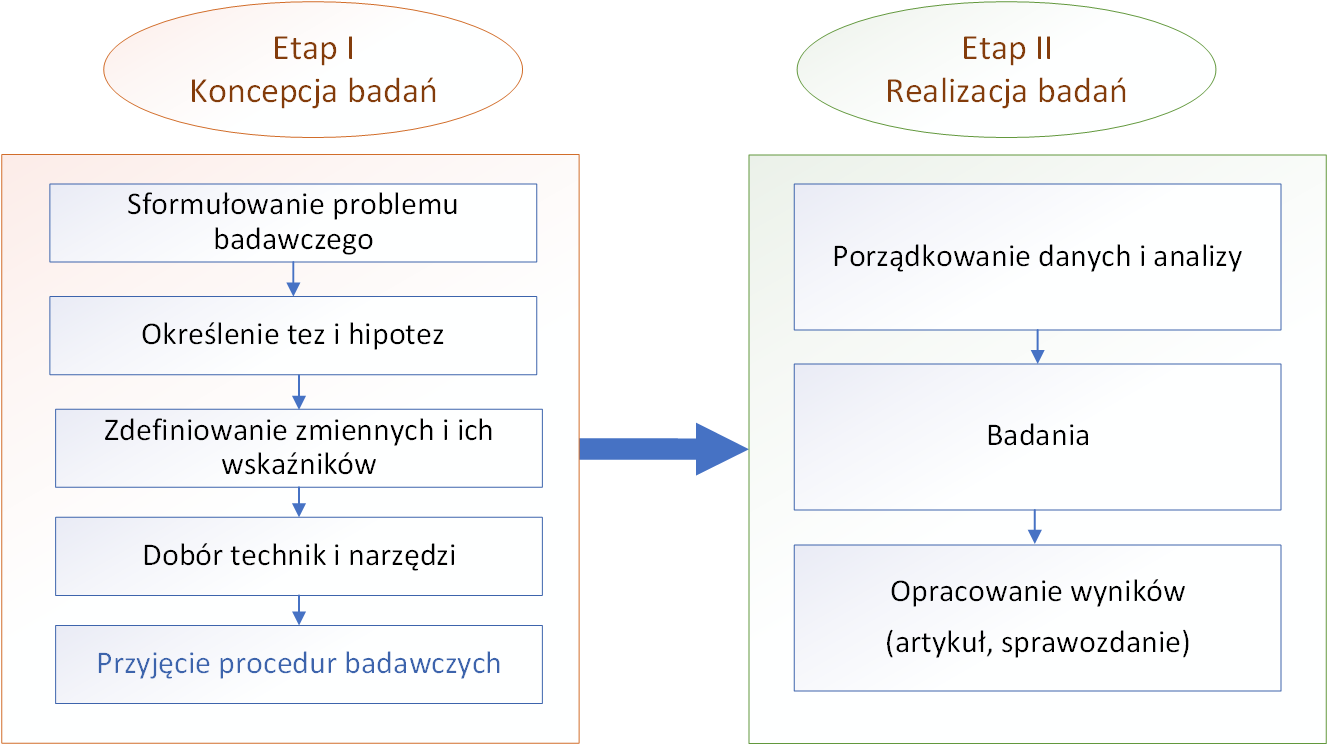
\includegraphics[width=1\textwidth,height=\textheight]{Rysunki/etapy_pracy_badawczej.png}
\caption{Etapy i czynności badań naukowych \label{etapy_badan}}
\end{figure}

Efektem udokumentowania przeprowadzonych badań najczęściej jest
napisanie artykułu naukowego. Uniwersalny schemat często wykorzystywany
podczas realizacji publikacji naukowej przedstawiono na rysunku
\ref{struktura_pub}.

\begin{figure}
\centering
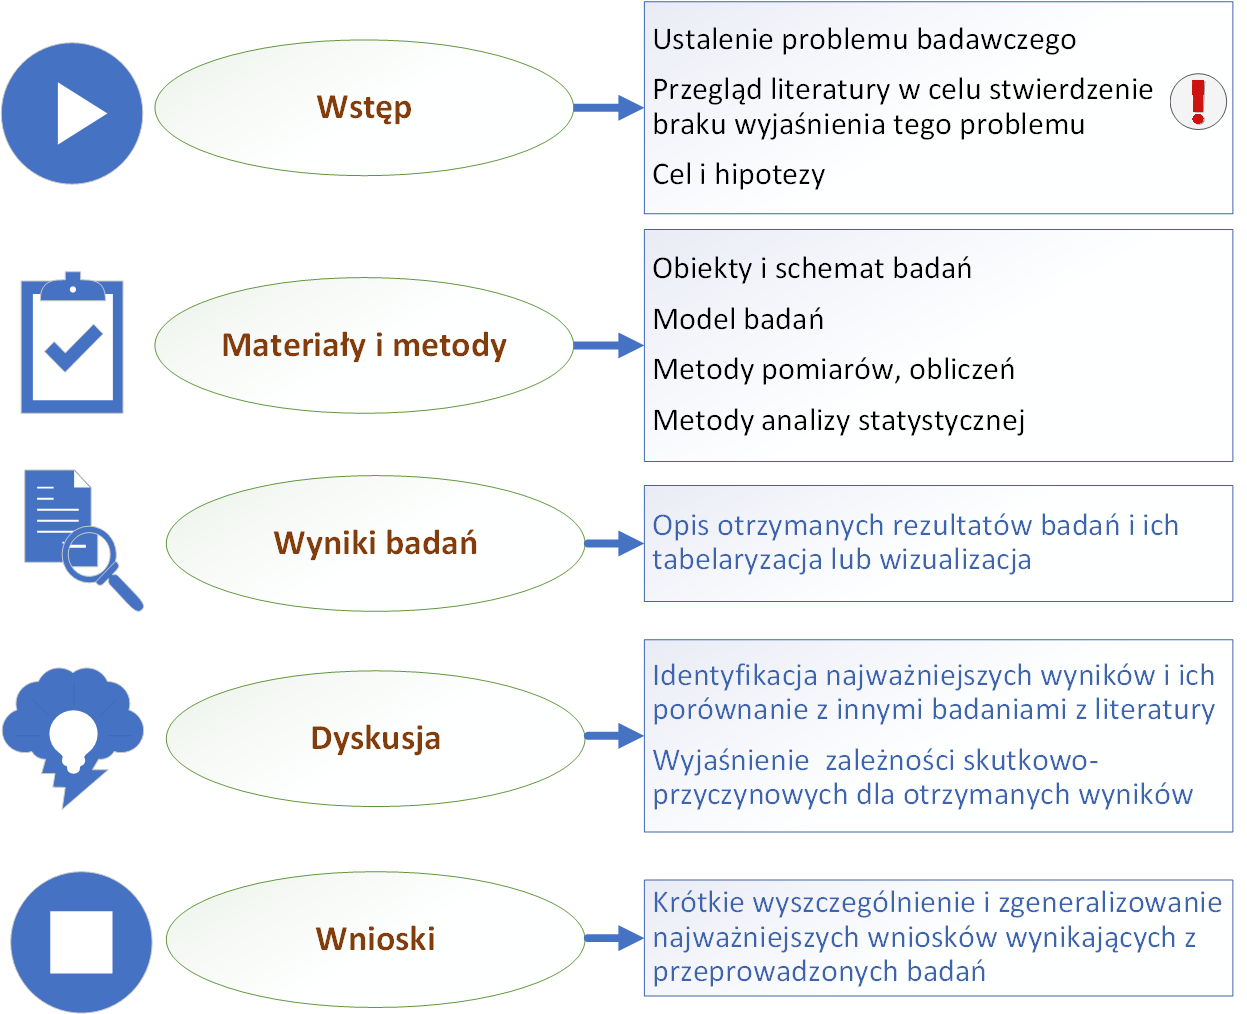
\includegraphics[width=1\textwidth,height=\textheight]{Rysunki/uklad_pracy_badawczej.png}
\caption{Uniwersalna struktuta publikacji naukowej
\label{struktura_pub}}
\end{figure}

Po ustaleniu problemu badawczego i tematu pracy, rozpoczyna się zwykle
etap pracy związany z poszukiwaniem literatury przedmiotu. Celem tego
etapu pracy jest stwierdzenie stanu wiedzy przeszłej i aktualnej
związanej z podjętym tematem badań, określenie brakujących luk i
możliwości ich wypełnienia oraz zasadności poszerzenia wiedzy z danego
obszaru badań (\protect\hyperlink{ref-cooper1986}{Cooper, 1986}) .

Przegląd literatury dotyczy najczęściej publikacji naukowych, które w
obowiązującym obecnie prawie (\protect\hyperlink{ref-dz.u.2019}{Dz. U.,
2019}) w rozumieniu ewaluacji (\protect\hyperlink{ref-pbn2020}{PBN,
2020}) określane są jako: - artykuł naukowy, - monografię naukową, -
rozdział w monografii naukowej.

Słownik Polskiej Bibliografii Naukowej
(\protect\hyperlink{ref-pbn2020}{PBN, 2020}) podaje następujące
definicje publikacji naukowych:

\begin{enumerate}
\def\labelenumi{\arabic{enumi}.}
\tightlist
\item
  Artykuł naukowy jest to recenzowany artykuł opublikowany w czasopiśmie
  naukowym albo w recenzowanych materiałach z międzynarodowych
  konferencji naukowych:
\end{enumerate}

\begin{itemize}
\tightlist
\item
  przedstawiający określone zagadnienie naukowe w sposób oryginalny i
  twórczy, problemowy albo przekrojowy;
\item
  opatrzony przypisami, bibliografią lub innym właściwym dla danej
  dyscypliny naukowej aparatem naukowym.
\end{itemize}

Artykułem naukowym jest również artykuł recenzyjny opublikowany w
czasopiśmie naukowym zamieszczonym w wykazie czasopism.

Artykułem naukowym nie jest: edytorial, abstrakt, rozszerzony abstrakt,
list, errata oraz nota redakcyjna.

\begin{enumerate}
\def\labelenumi{\arabic{enumi}.}
\setcounter{enumi}{1}
\tightlist
\item
  Monografia naukowa jest to recenzowana publikacja książkowa:
\end{enumerate}

\begin{itemize}
\tightlist
\item
  przedstawiająca określone zagadnienie naukowe w sposób oryginalny i
  twórczy;
\item
  opatrzona przypisami, bibliografią lub innym właściwym dla danej
  dyscypliny naukowej aparatem naukowym.
\end{itemize}

Monografią naukową jest również:

\begin{itemize}
\tightlist
\item
  recenzowany i opatrzony przypisami, bibliografią lub innym właściwym
  dla danej dyscypliny naukowej aparatem naukowym przekład na język
  polski dzieła istotnego dla nauki lub kultury albo na inny język
  nowożytny dzieła istotnego dla nauki lub kultury, wydanego w języku
  polskim;
\item
  edycja naukowa tekstów źródłowych.
\end{itemize}

Oceny poziomu naukowego prowadzonej działalności naukowej w zakresie
badań naukowych i prac rozwojowych dokonuje się z uwzględnieniem
następujących rodzajów osiągnięć naukowych
(\protect\hyperlink{ref-dz.u.2019}{Dz. U., 2019}):

\begin{enumerate}
\def\labelenumi{\arabic{enumi}.}
\item
  artykułów naukowych opublikowanych w czasopismach naukowych i w
  recenzowanych materiałach z międzynarodowych konferencji naukowych,
  zamieszczonych w wykazie tych czasopism i materiałów sporządzonym
  zgodnie z przepisami wydanymi na podstawie art. 267 ust. 2 pkt 2
  ustawy, zwanym dalej „wykazem czasopism'';
\item
  artykułów naukowych opublikowanych w czasopismach naukowych
  niezamieszczonych w wykazie czasopism;
\item
  monografii naukowych wydanych przez wydawnictwa zamieszczone w wykazie
  tych wydawnictw sporządzonym zgodnie z przepisami wydanymi na
  podstawie art. 267 ust. 2 pkt 2 ustawy, zwanym dalej „wykazem
  wydawnictw'';
\item
  monografii naukowych wydanych przez wydawnictwa niezamieszczone w
  wykazie wydawnictw, redakcji naukowych takich monografii i autorstwa
  rozdziałów w takich monografiach;
\item
  przyznanych patentów na wynalazki, praw ochronnych na wzory użytkowe i
  wyłącznych praw hodowców do odmian roślin.
\end{enumerate}

Proces publikowania wyników badań obecnie ulega ciągłej modyfikacji i
przyspieszeniu związanym z coraz większym dostępem do Internetu oraz
szybszemu procesowi przyjmowania i recenzji publikacji poprzez strony
własne Wydawnictw.

Szacuje się, że od 1996 roku opublikowano co najmniej 64 miliony
artykułów naukowych, a tempo wzrostu liczby nowo opublikowanych
artykułów \ref{pub_rocznie} ciągle ma tendencje wzrostową
(\protect\hyperlink{ref-curcic2023}{Curcic, 2023}).

\begin{figure}
\centering
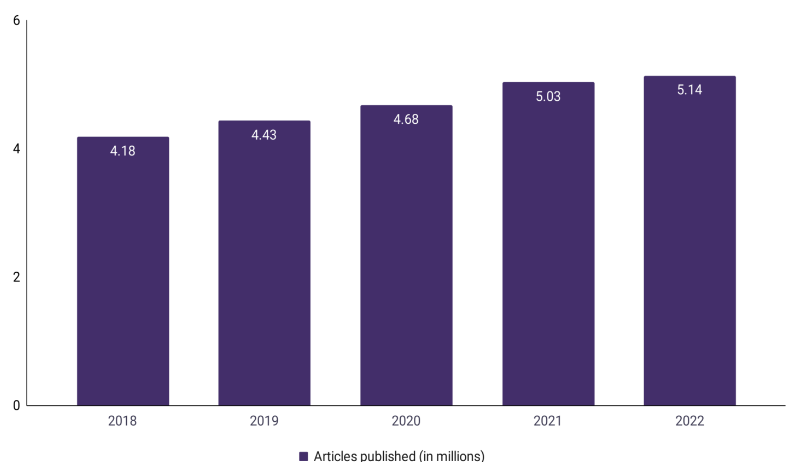
\includegraphics[width=1\textwidth,height=\textheight]{Rysunki/publikacje_rocznie.png}
\caption{Ilość publikowanych artykułów rocznie na świecie
\label{pub_rocznie}}
\end{figure}

Z raportu \href{https://ncses.nsf.gov/indicators}{S\&E - Science and
Engineering Indicators} wynika, że roczny przyrost ilości publikacji na
świecie artykułów naukowo-technicznych wyniósł 4\% w latach 2010-2020
(\protect\hyperlink{ref-curcic2023}{Curcic, 2023}). Na rysunku
\ref{Ilosc_publikacji} zestawiono ilość artykułów naukowo-technicznych
opublikowanych ze wszystkich obszarów nauki na świecie oraz w 15
największych krajach w latach 2010 i 2020.

\begin{figure}
\centering
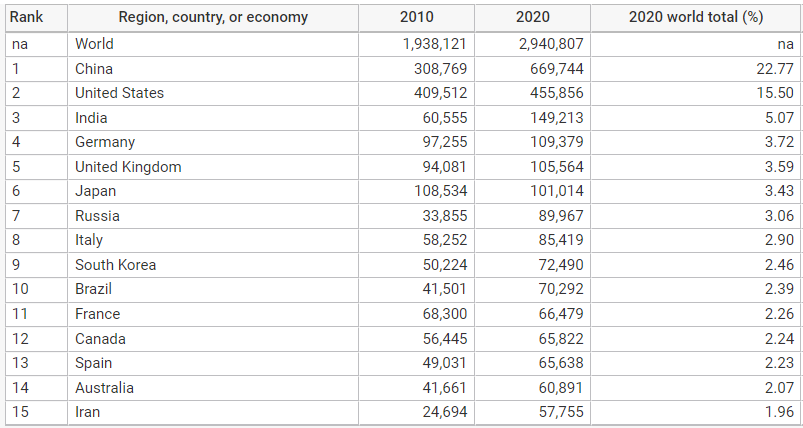
\includegraphics[width=1\textwidth,height=\textheight]{Rysunki/ilosc_opublikowanych_artykulow.png}
\caption{Ilość opublikowanych artykułów naukowo-technicznych
\label{Ilosc_publikacji}}
\end{figure}

Graficzny obraz przyrostu publikowanych artykułów naukowo-technicznych
od roku 1996 przedstawiono na rysunku \ref{grafika_pub_nauk_tech}.
Uwidacznia się na nim wyraźne ogólna tendencja przyrostu publikacji na
świecie, a z pośród analizowanych krajów szczególnie jest to widoczne w
Chinach.

\begin{figure}
\centering
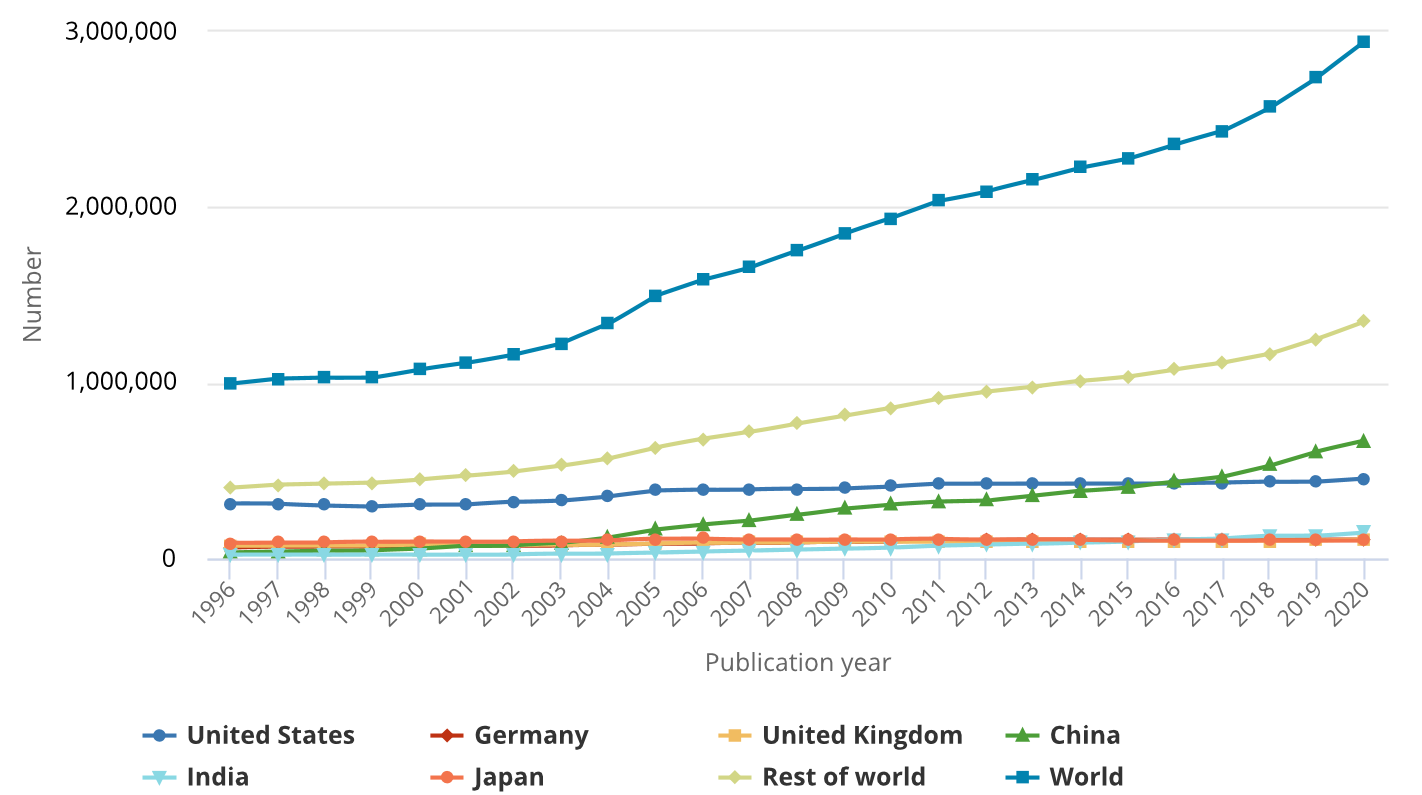
\includegraphics[width=1\textwidth,height=\textheight]{Rysunki/ilosc_pub_graf.png}
\caption{Trendy w ilosci publikowanych artykułów naukowo-technicznych
\label{grafika_pub_nauk_tech}}
\end{figure}

Ilość publikowanych artykułów na świecie koreluje dodatnio ze
wzrastająca ilością czasopism akademickich. W 2020 roku odnotowano 46,7
tys. czasopism \ref{liczba_czasopism}, a ciągu ostatnich 10 lat liczba
ich wzrosła o 29\% (\protect\hyperlink{ref-curcic2023}{Curcic, 2023}).

\begin{figure}
\centering
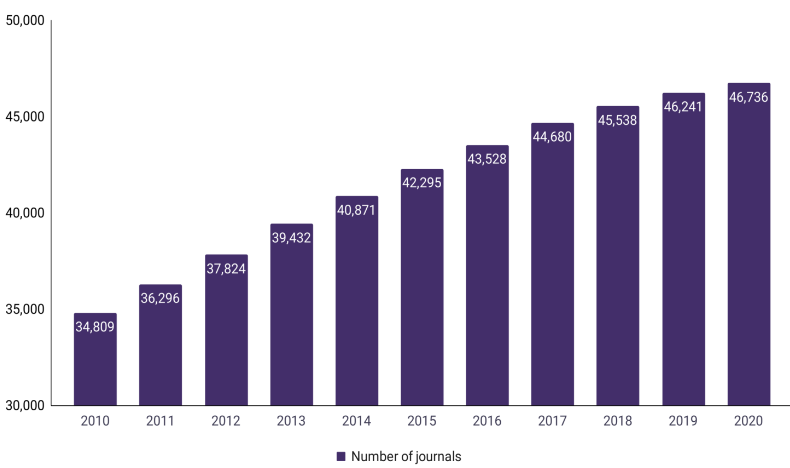
\includegraphics[width=1\textwidth,height=\textheight]{Rysunki/liczba_czasopism.png}
\caption{Ilość czasopism akademickich na świaecie
\label{liczba_czasopism}}
\end{figure}

O wymiarze publikowanych prac naukowych na świecie z zakresu nauk
fizycznych, chemicznych oraz nauk o życiu i środowisku można się
dowiedzieć ze strony \href{https://natureindex.com}{natureindex.com}. Na
podstawie danych (od 1 czerwca 2021 do 31 maja 2022) z tej strony na
rysunku \ref{pub_swiat} wyszczególniono kraje o największej ilości
publikacji. Dane te uwidaczniają, że niekwestionowanymi liderami w tych
obszarach badań są USA oraz Chiny.

\begin{figure}
\centering

\includegraphics{Rysunki/figures/unnamed-chunk-21-1.pdf}
\caption{Kraje o największej ilości publikacji z analizowanego obszarów
badań. \label{pub_swiat}}
\end{figure}

Ilość prac naukowych z tych obszarów badawczych w Europie przedstawiono
na rysunku \ref{pub_europa}, gdzie uwidacznia się, że na kontynencie
europejskim liderami są Wielka Brytania i Niemcy.

\begin{figure}
\centering

\includegraphics{Rysunki/figures/unnamed-chunk-22-1.pdf}
\caption{Ilość publikacji w Europie z analizowanego obszaru badań.
\label{pub_europa}}
\end{figure}

W Polsce opublikowano w tym okresie z tego obszaru badań 906 artykułów
naukowych z pośród których 296 były napisane ze współautorami z innych
krajów. Udział publikacji w poszczególnych obszarach badań przedstawiono
na rysunku \ref{polska_subject}.

\begin{figure}
\centering
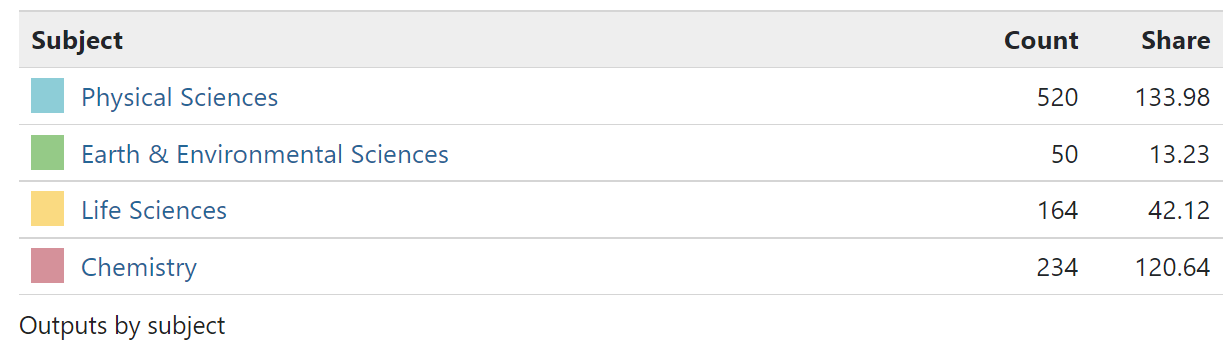
\includegraphics{Rysunki/polska_subject.png}
\caption{Ilość publikacji w zależności od obszaru badań.
\label{polska_subject}}
\end{figure}

W latach 2017--2021 opublikowano w Polsce około 619 tys. prac naukowych,
z których większość (67\%) stanowiły artykuły, 29\% -- rozdziały w
monografiach, a pozostałe 4\% -- monografie naukowe
(\protect\hyperlink{ref-pwn2023}{PWN, 2023}).

Tak znaczący przyrost ilości artykułów naukowych nasilają problemy z ich
przeglądem i oceną, która ma na celu znalezienie pytań bez odpowiedzi
lub nierozwiązanych problem w danej dziedzinie, który odzwierciedla brak
istniejących badań w danej obszarze badań.

W publikacjach naukowych znaczną część literatury podaje się na początku
pracy, aby wskazać kierunek pytań badawczych i hipotez
(\protect\hyperlink{ref-creswell2013}{Creswell, 2013}) . Wykonywanie
takich przeglądów standardowymi ``ręcznymi'' metodami jest coraz
bardziej czasochłonne i mało efektywne, dlatego metody i narzędzia data
science umożliwiają ten etap pracy naukowej znacznie przyspieszyć i
zwiększyć jego efektywność.

\FloatBarrier
\newpage
\fancyhead[C]{Metodyka badań}

\hypertarget{metody-badaux144}{%
\section{Metody badań}\label{metody-badaux144}}

W pracy własnej wykorzystano narzędzia z obszaru dziedziny Data Science,
dlatego poniżej zdefiniowano ten obszar wiedzy. Data Science (polska
nazwa - danologia) to interdyscyplinarna dziedzina generalnie zajmująca
się analizą danych (pozyskiwaniem, eksploracją, wizualizowaniem i
wyciąganiem z takich analiz wniosków. W szeroko rozumianym obszarze Data
Science wykorzystuje się metody oparte na programowaniu, analizie
statystycznej, uczeniu maszynowym (Machine Learning), sztucznej
inteligencji, sieci neuronowych, czy analizie dużych baz danych (Big
Data).

\hypertarget{narzux119dzia-data-science-wykorzystane-w-pracy}{%
\subsection{Narzędzia Data Science wykorzystane w
pracy}\label{narzux119dzia-data-science-wykorzystane-w-pracy}}

\begin{itemize}
\tightlist
\item
  Program Python
\item
  Program R
\item
  RStudio
\item
  R Markdown
\item
  LaTeX
\item
  Zotero.
\end{itemize}

\hypertarget{program-python-python.org}{%
\subsubsection{\texorpdfstring{Program Python
\href{https://www.python.org}{python.org}}{Program Python python.org}}\label{program-python-python.org}}

Python określany jest jako wysoko poziomowy, dynamiczny językiem
ogólnego przeznaczenia rys. \ref{python}.

\begin{figure}
\centering

\includegraphics[width=0.8\textwidth,height=\textheight]{Rysunki/python.png}
\caption{Program Python \label{python}}
\end{figure}

Obecnie jest najbardziej popularnym i najszybciej rozwijającym się
językiem programowania na świecie według portalu
\href{https://www.tiobe.com/tiobe-index/}{TIOBE Index} rys.
\ref{ranking_prog}.

\begin{figure}
\centering
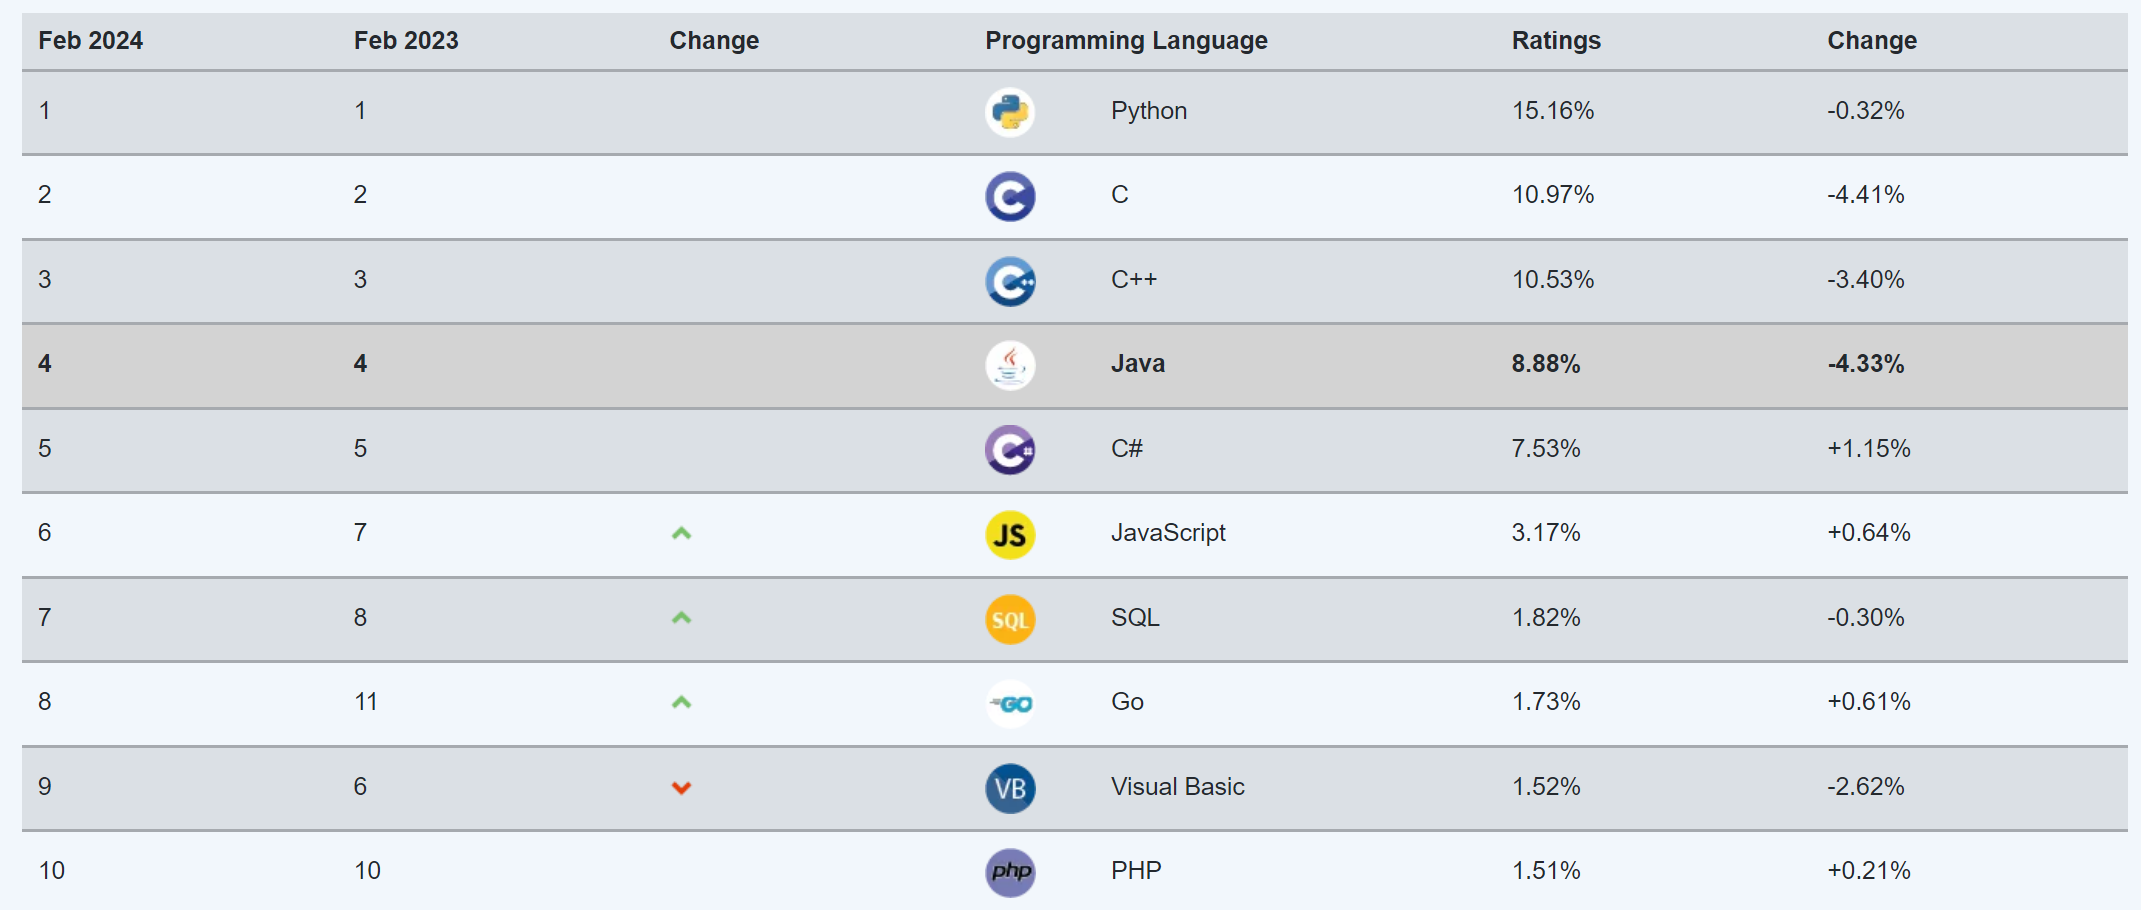
\includegraphics[width=1\textwidth,height=\textheight]{Rysunki/ranking_programow.png}
\caption{Ranking programów TIOBE Index \label{ranking_prog}}
\end{figure}

Pierwsza wersja Pythona ukazała się na początku 1991 roku i zaliczany
jest do kategorii oprogramowania Open Source. Do głównych zalet Pythona
zalicza się nowoczesną składnię języka z opcją wyboru różnych
paradygmatów programowania (funkcyjnego, obiektowego, reaktywnego), dużą
i przyjazną społeczność, bogaty zbiór wbudowanych i przenośnych opcji,
sprawną komunikację z innymi częściami aplikacji, współpracę pomiędzy
najważniejszymi platformami - Windowsa oraz Linuxa
(\protect\hyperlink{ref-comarch2023}{Comarch, 2023}).

\hypertarget{program-r-r-project.org}{%
\subsubsection{\texorpdfstring{Program R
\href{https://www.r-project.org}{r-project.org}}{Program R r-project.org}}\label{program-r-r-project.org}}

R jest oprogramowaniem o otwartym kodzie źródłowym, dostępnym w Uniksie,
Linuksie, a także systemach macOS i Windows
(\protect\hyperlink{ref-wickham2018}{Wickham i Grolemund, 2018}).

Logo tego programu przedstawiono na rysunku \ref{r_logo.svg}.

\begin{figure}
\centering

\includegraphics[width=0.2\textwidth,height=\textheight]{Rysunki/r_logo_svg.png}
\caption{Logo programu R. \label{r_logo.svg}}
\end{figure}

Pierwsza wersja R została napisana w roku 1991 przez Roberta Gentlemana
i Rossa Ihake˛ (znanych jako R\&R), pracujących na Wydziale Statystyki
Uniwersytetu w Auckland. Program R jest projektem GNU opartym na
licencji GNU GPL, co oznacza, iż jest zupełnie darmowy zarówno do
zastosowań edukacyjnych, jak i biznesowych
(\protect\hyperlink{ref-biecek2017}{Biecek, 2017}).

Język R jest językiem interpretowanym, a nie kompilowanym, oznacza to,
że program w nim napisany nie będzie tak szybki jak np. program napisany
w C++. Język R ma elastyczną składnię i pozwala użytkownikom na
definiowanie własnych, dowolnie złożonych, funkcji
(\protect\hyperlink{ref-guxf3recki2011}{Górecki, 2011}).

R wykorzystuje się do obliczeń statystyczno-matematycznych, umożliwia on
również tworzenie zaawansowanych wykresów.

Po zainstalowaniu podstawowego środowiska R mamy już dostęp do wielu
użytecznych funkcjonalności, jednak możliwości pracy w R zwiększają się
bardzo po zainstalowaniu dodatkowych pakietów (package). Szacuje się, że
2020 roku dostępnych ich było około 16 tysięcy
\href{https://en.wikipedia.org/wiki/R_package}{wikipedia.org}.

\hypertarget{rstudio-rstudio.com}{%
\subsubsection{\texorpdfstring{RStudio
\href{https://www.rstudio.com}{rstudio.com}}{RStudio rstudio.com}}\label{rstudio-rstudio.com}}

Istnieje kilka graficznych interfejsów dla programu R, wśród nich
najbardziej popularnym jest RStudio (rys. \ref{rstudio}).

RStudio określa się jako zintegrowane środowisko programistyczne (IDE)
dla języka R.

\begin{figure}
\centering

\includegraphics[width=0.3\textwidth,height=\textheight]{Rysunki/r_studio.png}
\caption{Logo RStudio\label{rstudio}}
\end{figure}

RStudio zawiera konsolę, edytor podświetlający składnię i obsługuje
bezpośrednie wykonywanie kodu, a także narzędzia do tworzenia wykresów,
historii, debugowania i zarządzania przestrzenią roboczą (rys.
\ref{rstudio_edytor}).

\begin{figure}
\centering
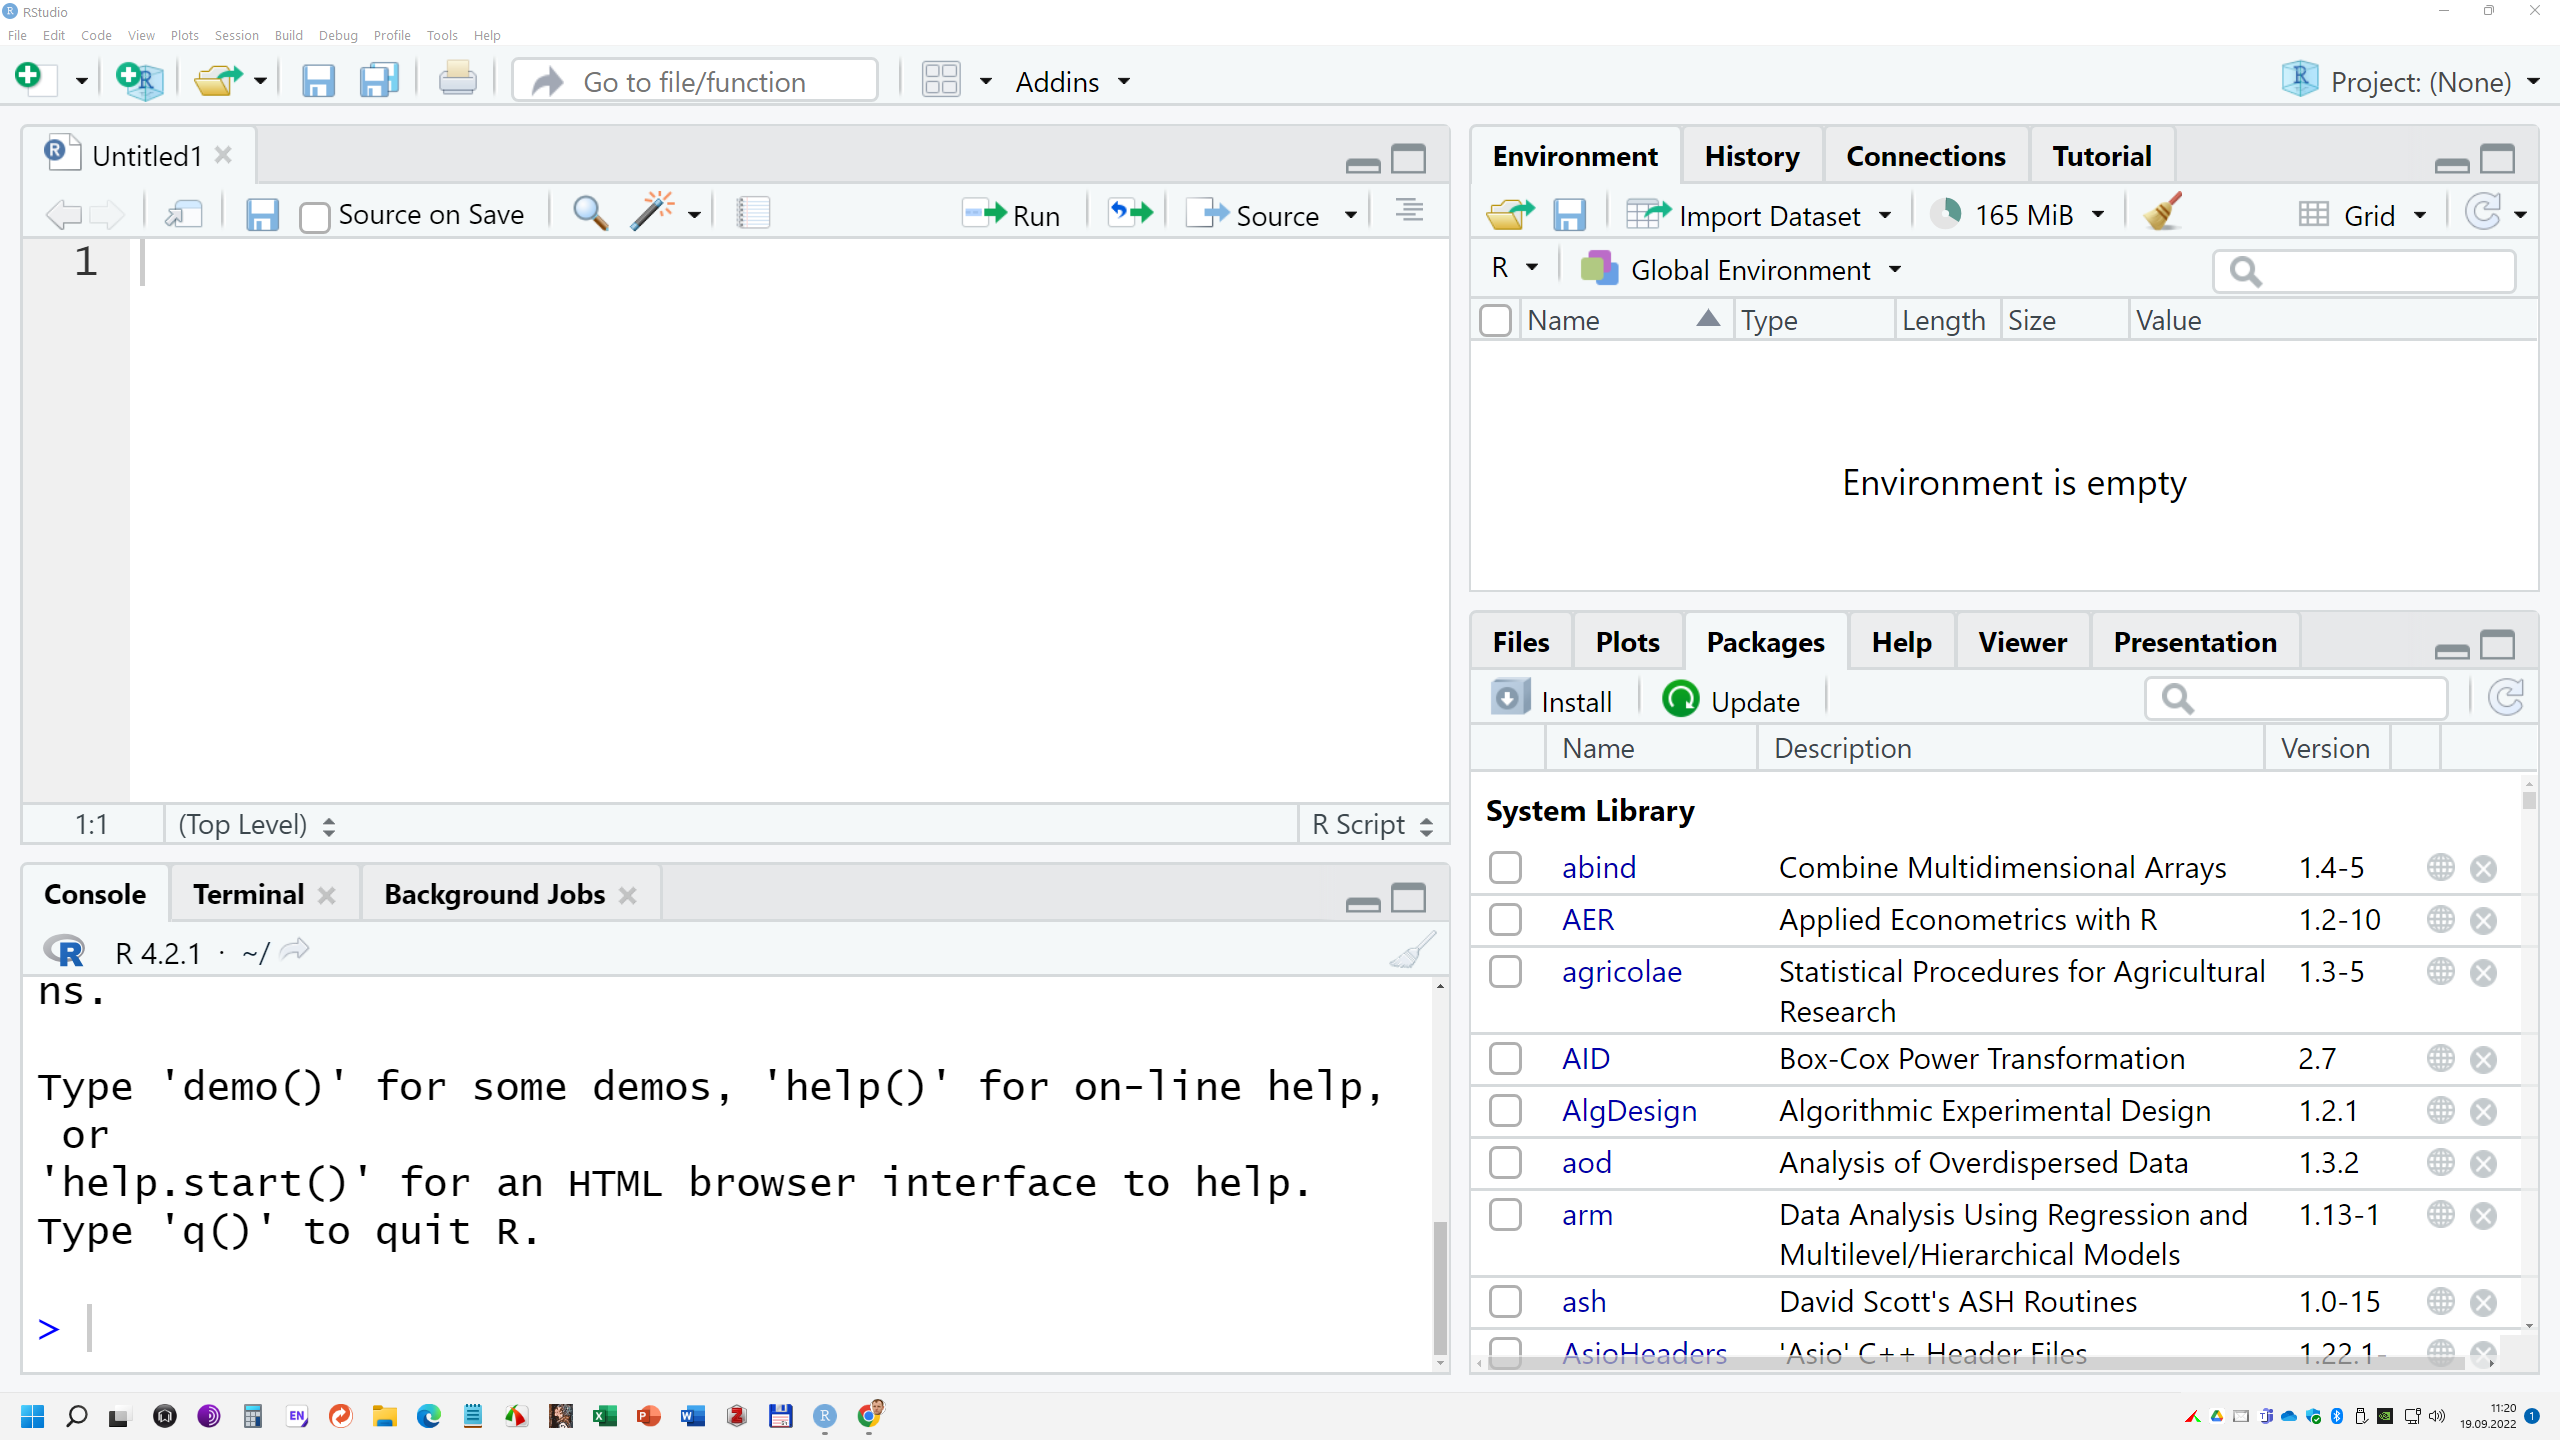
\includegraphics{Rysunki/rstudio_edytor.png}
\caption{RStudio\label{rstudio_edytor}}
\end{figure}

\hypertarget{r-markdown-rmarkdown.com}{%
\subsubsection{\texorpdfstring{R Markdown
\href{https://rmarkdown.rstudio.com/}{rmarkdown.com}}{R Markdown rmarkdown.com}}\label{r-markdown-rmarkdown.com}}

Rmarkdown to narzędzie do tworzenia dynamicznych dokumentów i zestawień.
Język znaczników, którego celem jest jak największe uproszczenie
tworzenia i formatowania tekstu
\href{https://en.wikipedia.org/wiki/Markdown}{wikipedia.org}.

\begin{figure}
\centering

\includegraphics[width=0.4\textwidth,height=\textheight]{Rysunki/r_markdown.png}
\caption{Rmarkdown\label{rmarkdown}}
\end{figure}

Biblioteka rmarkdown wraz z formatem R Markdown pozwala na przygotowanie
estetycznie wyglądających raportów, a dokumenty otrzymywane w wyniku ich
tworzenia są dynamiczne ponieważ istnieje w nich możliwość zagnieżdżania
języka R (\protect\hyperlink{ref-strus2017}{Struś, 2017}).

\hypertarget{latex-latex-project.org}{%
\subsubsection{\texorpdfstring{LaTeX
\href{https://www.latex-project.org/}{latex-project.org}}{LaTeX latex-project.org}}\label{latex-latex-project.org}}

LaTeX to oprogramowanie do zautomatyzowanego składu tekstu, a także
związany z nim język znaczników, służący do formatowania dokumentów
tekstowych i tekstowo-graficznych
\href{https://pl.wikipedia.org/wiki/LaTeX}{wikipedia.org}.

\begin{figure}
\centering

\includegraphics[width=0.4\textwidth,height=\textheight]{Rysunki/LaTeX.png}
\caption{LaTeX\label{latex}}
\end{figure}

Oprogramowanie to określane jest także jako zestaw makropoleceń
stanowiących nadbudowę nad systemem składu TEX, automatyzujących wiele
czynności związanych z procesem poprawnego składania tekstu
(\protect\hyperlink{ref-ziemkiewicz2013}{Ziemkiewicz i Karłowska-Pik,
2013}).

LATeX w swojej naturze odpowiada metodologii WYSIWYM, gdzie autor
określa jedynie strukturę logiczną i treść dokumentu, pozostawiając w
rękach automatycznego systemu zagadnienia dotyczące wyglądu i
odpowiedniego rozmieszczenia elementów na stronie
(\protect\hyperlink{ref-borkowski2015}{Borkowski i Przybylski, 2015}).

\hypertarget{bazy-danych-indeksujux105ce-publikacje-naukowe}{%
\subsection{Bazy danych indeksujące publikacje
naukowe}\label{bazy-danych-indeksujux105ce-publikacje-naukowe}}

Obecnie pracownicy nauki korzystają najczęściej z baz danych, takich jak
Google Scholar, Lens, Semantic Scholar, Scopus, Web of Science i
ResearchGate w celu uzyskania dostępu i ocenienia literatury naukowej.
Pomiedzy tymi bazami zauważa się pewne podobieństwa istnieją jednak
również istotne różnice pod względem ich zasięgu, zakresu, możliwości
wyszukiwania i wskaźników cytowań.

Poniżej przedstawiono krótka charakterystykę wymienionych baz
indeksujących.

\href{scholar.google.com}{Google Scholar} najpopularniejsze narzędzie ze
względu na to, że jest szybkie, bezpłatne i wszechstronne. Usługę tą
rozpoczęto w listopadzie 2004 r. Kataloguje piśmiennictwo akademickie z
różnych dziedzin i źródeł, takich jak książki, prace dyplomowe, artykuły
z czasopism, materiały konferencyjne i preprinty rys.
\ref{gogle_scholar}. Obejmuje ona szeroki zakres publikacji, w tym
takie, które mogą nie być indeksowane przez inne bazy danych.

\begin{figure}
\centering

\includegraphics[width=1\textwidth,height=\textheight]{Rysunki/google_scholar.png}
\caption{Google Scholar \label{gogle_scholar}}
\end{figure}

\href{lens.org}{Lens} darmowy i otwarty zasób służący do wyszukiwania,
analizowania i zarządzania danymi patentowymi i naukowymi rys.
\ref{lens}. Umożliwia użytkownikom wyszukiwanie i dostęp do ponad 200
milionów dokumentów patentowych i 100 milionów publikacji akademickich z
różnych źródeł.

\begin{figure}
\centering

\includegraphics[width=1\textwidth,height=\textheight]{Rysunki/lens.png}
\caption{Lens \label{lens}}
\end{figure}

\FloatBarrier
\newpage
\fancyhead[C]{Wyniki badań i dyskusja}

\hypertarget{wyniki-badaux144-i-dyskusja}{%
\section{Wyniki badań i dyskusja}\label{wyniki-badaux144-i-dyskusja}}

\hypertarget{przygotowanie-ux15brodowiska-do-pracy-w-r}{%
\subsection{Przygotowanie środowiska do pracy w
R}\label{przygotowanie-ux15brodowiska-do-pracy-w-r}}

\hypertarget{instalacja-r}{%
\subsubsection{Instalacja R}\label{instalacja-r}}

Rozpoczęcie pracy z R związane jest z zainstalowaniem tego programu.
Jest to darmowe środowisko programistyczne, które kompiluje się i działa
na wielu różnych platformach UNIX, Windows i MacOSa. Najlepszą opcją
jest pobranie tego programu z oficjalnej strony projektu -
\href{https://www.r-project.org/}{r-project.org} (rys. \ref{strona_r}).

\begin{figure}
\centering
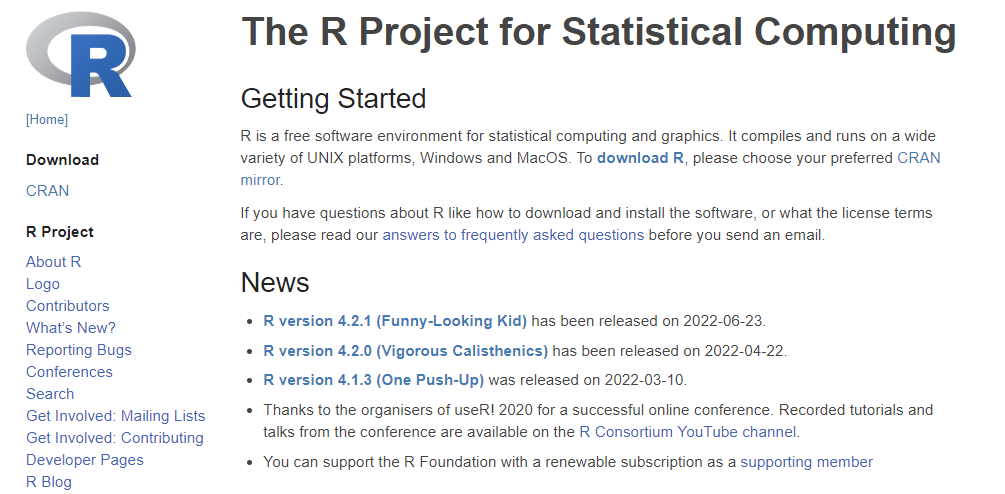
\includegraphics{Rysunki/strona_r.png}
\caption{Strona www projektu R \label{strona_r}}
\end{figure}

\hypertarget{instalacja-rstudio}{%
\subsubsection{Instalacja Rstudio}\label{instalacja-rstudio}}

Po instalacji R można zainstalować graficzny interfejs dla programu R w
postaci programu Rstudio. Na oficjalnej stronie
\href{https://www.rstudio.com}{Rstudio} można pobrać darmową wersję tego
programu (rys. \ref{pobieranie_rstudio}).

\begin{figure}
\centering
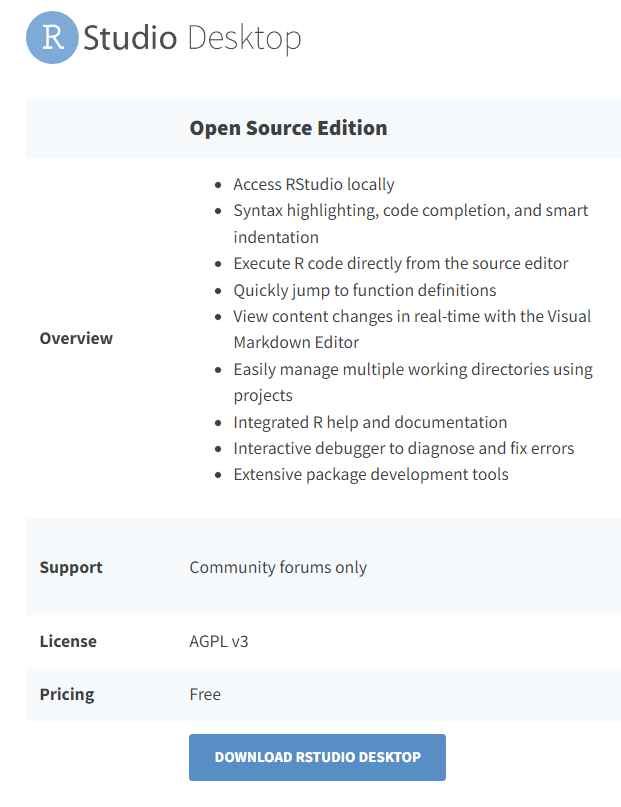
\includegraphics[width=0.6\textwidth,height=\textheight]{Rysunki/pobieranie_rstudio.png}
\caption{Pobieranie darmowej wersji programu Rstudio
\label{pobieranie_rstudio}}
\end{figure}

\hypertarget{instalacja-pakietu-rmarkdown}{%
\subsubsection{\texorpdfstring{Instalacja pakietu
\textbf{rmarkdown}}{Instalacja pakietu rmarkdown}}\label{instalacja-pakietu-rmarkdown}}

Oficjalnym źródłem dokumentacji dla pakietów do języka R jest
\href{https://cran.r-project.org/web/packages/available_packages_by_name.html}{CRAN}
( Comprehensive R Archive Network), gdzie jest umieszczony spis
dostępnych pakietów.

Pakiety w Rstudio można instalować zarówno z poziomu konsoli poprzez
użycie właściwej komendy. Poniżej zapisano przykładową funkcję
instalacyjną dla pakietu rmarkdown :

\texttt{install.packages("rmarkdown")}

Możliwe jest także zainstalowanie pakietów poprzez panel z zakładką
pakiety. Pliki R Markdown to pliki tekstowe, które zazwyczaj mają
rozszerzenie \texttt{.Rmd}.

Pakiet R \texttt{rmarkdown} jest biblioteką, która przetwarza i
konwertuje pliki \texttt{.Rmd} do wielu różnych formatów.

W pakiecie rmarkdown domyślnie zawarty jest także program pandoc służący
do konwertowania dokumentów z formatów znaczników do wielu innych
formatów, takich jak \texttt{.docx}, \texttt{.pdf} itd. Pandoc dodaje
także funkcjonalność w języku bazowym markdown umożliwiajacą obsługę
bardziej złożonych wyjść.

\hypertarget{instalowanie-latex-tinytex-dla-tworzenia-pdf}{%
\subsubsection{Instalowanie LaTeX (TinyTeX) dla tworzenia
PDF}\label{instalowanie-latex-tinytex-dla-tworzenia-pdf}}

Przy tworzeniu dokumentów formatu pdf niezbędne jest zainstalowanie
LaTeXa. Dostępnych jest kilka opcji zainstalowania osobnych programów
obsługujących składnie LaTeXa jak MiKTeX, MacTeX i TeX Live, jednak
zalecane jest, żeby przy używaniu pakietu rmardown zainstalować pakiet
tinytex:

\texttt{install.packages("tinytex")}

\hypertarget{instalacja-pakietu-knitr}{%
\subsubsection{\texorpdfstring{Instalacja pakietu
\textbf{knitr}}{Instalacja pakietu knitr}}\label{instalacja-pakietu-knitr}}

Narzędzie to przeznaczone jest do dynamicznego generowania raportów w R
przy użyciu technik Literate Programming. (ang. programowanie piśmienne)
(\protect\hyperlink{ref-xie2022}{Xie, 2022}).

\begin{figure}
\centering

\includegraphics[width=0.27\textwidth,height=\textheight]{Rysunki/knit-logo.png}
\caption{Logo pakietu knitr \label{knit_logo}}
\end{figure}

Jak wskazuje logo pakietu knitr (rys. \ref{knit_logo}) jest to narzędzie
do spajania i generowania dynamicznych raportów w R. Knitr pozwala na
proste łączenie kodów R oraz ich opisów. Takie połączenie może być
wykorzystane zarówno do dokumentowania kodu, do zapewnienia
powtarzalności analiz jak i do automatycznego generowania raportów
(\protect\hyperlink{ref-xie2015}{Xie, 2015}).

Struś (\protect\hyperlink{ref-strus2017}{2017}) określa rolę pakietu
knitr jako silnika do generowania dynamicznych raportów w R, który
egzekwuje kod i tworzy nowy dokument markdown. MD, który zawiera kod i
wynik działania samego kodu.

\hypertarget{tworzenie-pliku-r-mardown-w-rstudio}{%
\subsection{Tworzenie pliku R Mardown w
RStudio}\label{tworzenie-pliku-r-mardown-w-rstudio}}

Po otwarciu programu RStudio uwidacznia się układ panelowy (rys.
\ref{panele_rstudio} ), gdzie rozmieszczenie poszczególnych paneli można
ustawiać w globalnych opcjach programu (rys. \ref{uklad_paneli}).

\begin{figure}
\centering
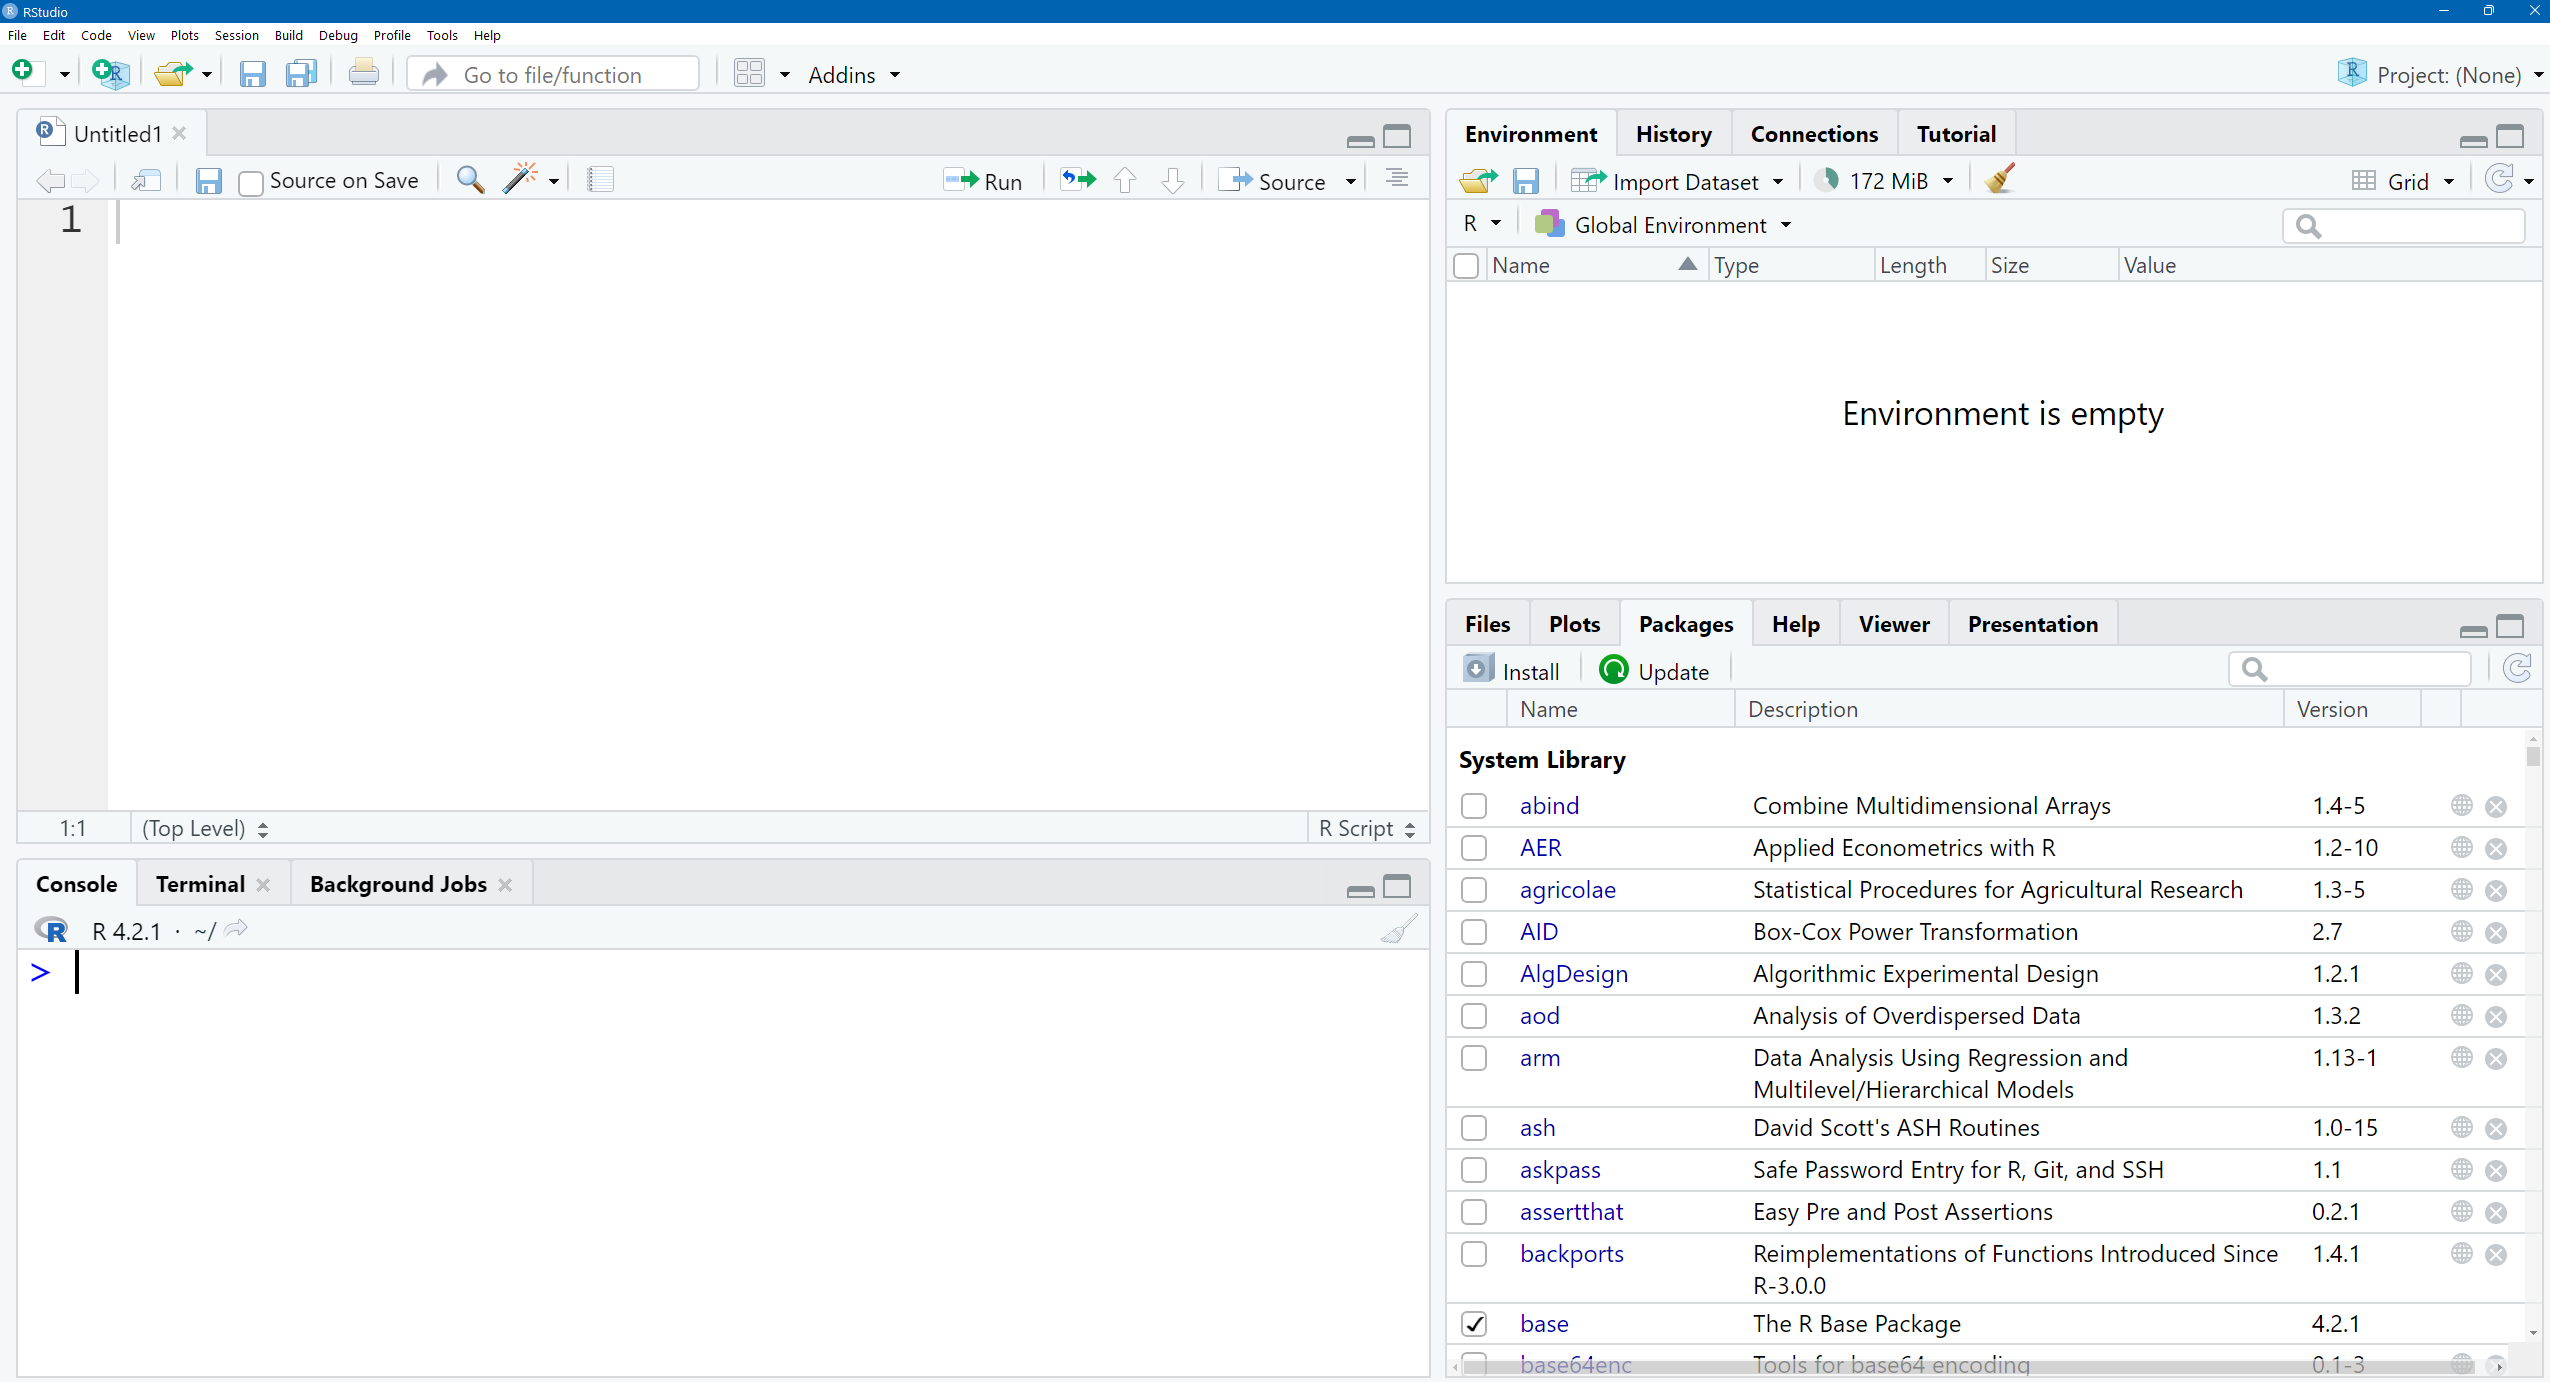
\includegraphics[width=0.8\textwidth,height=\textheight]{Rysunki/panele_rstudio.png}
\caption{Panelowy układ programu RStudio \label{panele_rstudio}}
\end{figure}

\begin{figure}
\centering
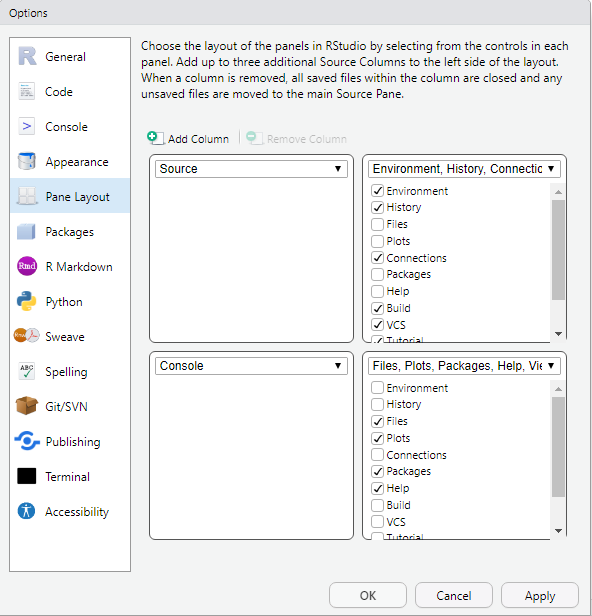
\includegraphics[width=0.4\textwidth,height=\textheight]{Rysunki/ustawienie_paneli_rstudio.png}
\caption{Ustawianie rozmieszczenia paneli w RStudio
\label{uklad_paneli}}
\end{figure}

W panelu edycji plików istnieje możliwość utworzenie pliku .Rmd, poprzez
otwarcie w menu File → New File → R Markdown (rys. \ref{plik_Rmd}).

\begin{figure}
\centering
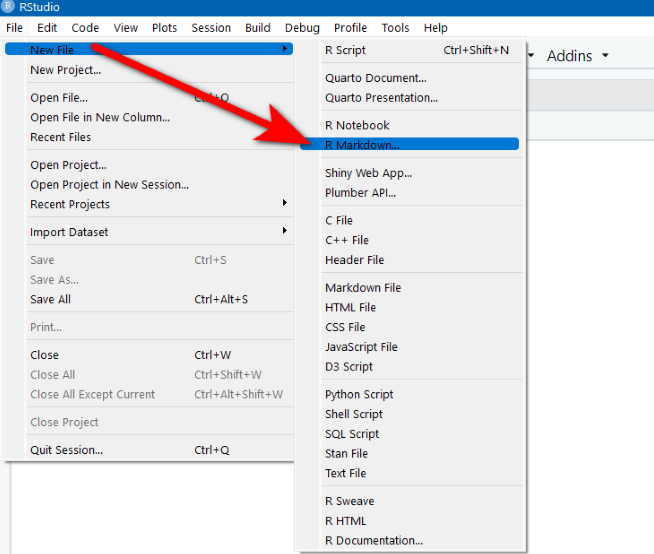
\includegraphics[width=0.65\textwidth,height=\textheight]{Rysunki/plik_Rmd.png}
\caption{Utworzenie pliku R markdown \label{plik_Rmd}}
\end{figure}

Zalecaną dobrą praktyką jest jednak utworzenie nowego projektu gdzie w
katalogu tego projektu zamieszczane są wszystkie pliki związane z
wykonywanym projektem (rys. \ref{nowy_projekt}, \ref{nowy_projekt_okno},
\ref{nowy_projekt_katalog}).

\begin{figure}
\centering
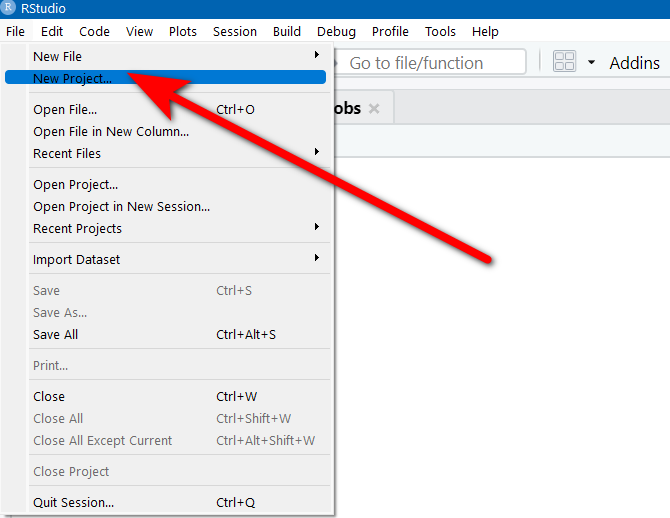
\includegraphics[width=0.65\textwidth,height=\textheight]{Rysunki/nowy_projekt.png}
\caption{Zakładanie nowego projektu \label{nowy_projekt}}
\end{figure}

\begin{figure}
\centering
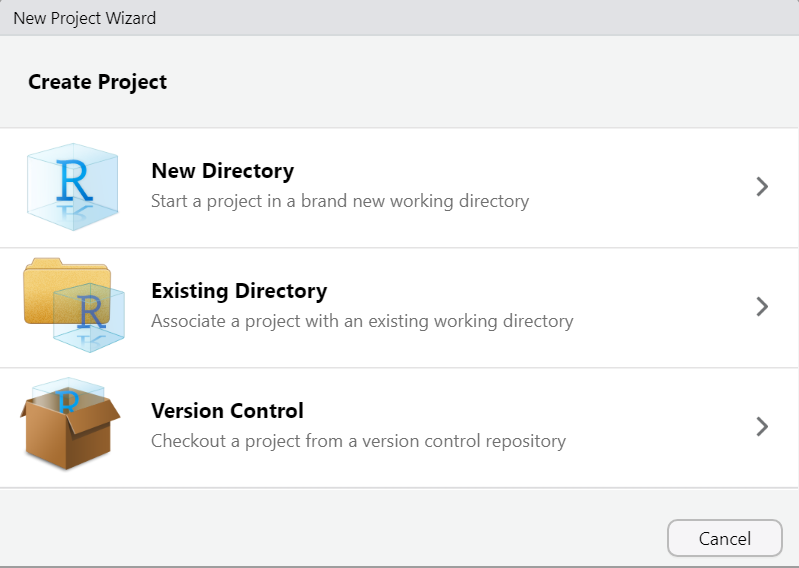
\includegraphics[width=0.6\textwidth,height=\textheight]{Rysunki/nowy_projekt_okno.png}
\caption{Okno nowego projektu \label{nowy_projekt_okno}}
\end{figure}

\begin{figure}
\centering
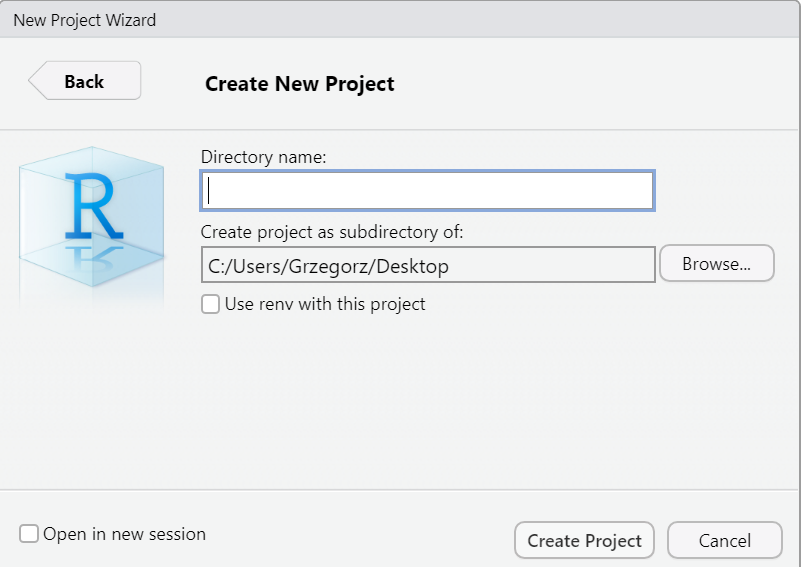
\includegraphics[width=0.6\textwidth,height=\textheight]{Rysunki/nowy_projekt_katalog.png}
\caption{Ustawienie docelowego katalogu projektu
\label{nowy_projekt_katalog}}
\end{figure}

W strukturze układu projektu możliwe jest tworzenie różnego rodzaju
plików w tym także plików .Rmd (rys. \ref{nowy_projekt_rmd}).

\begin{figure}
\centering
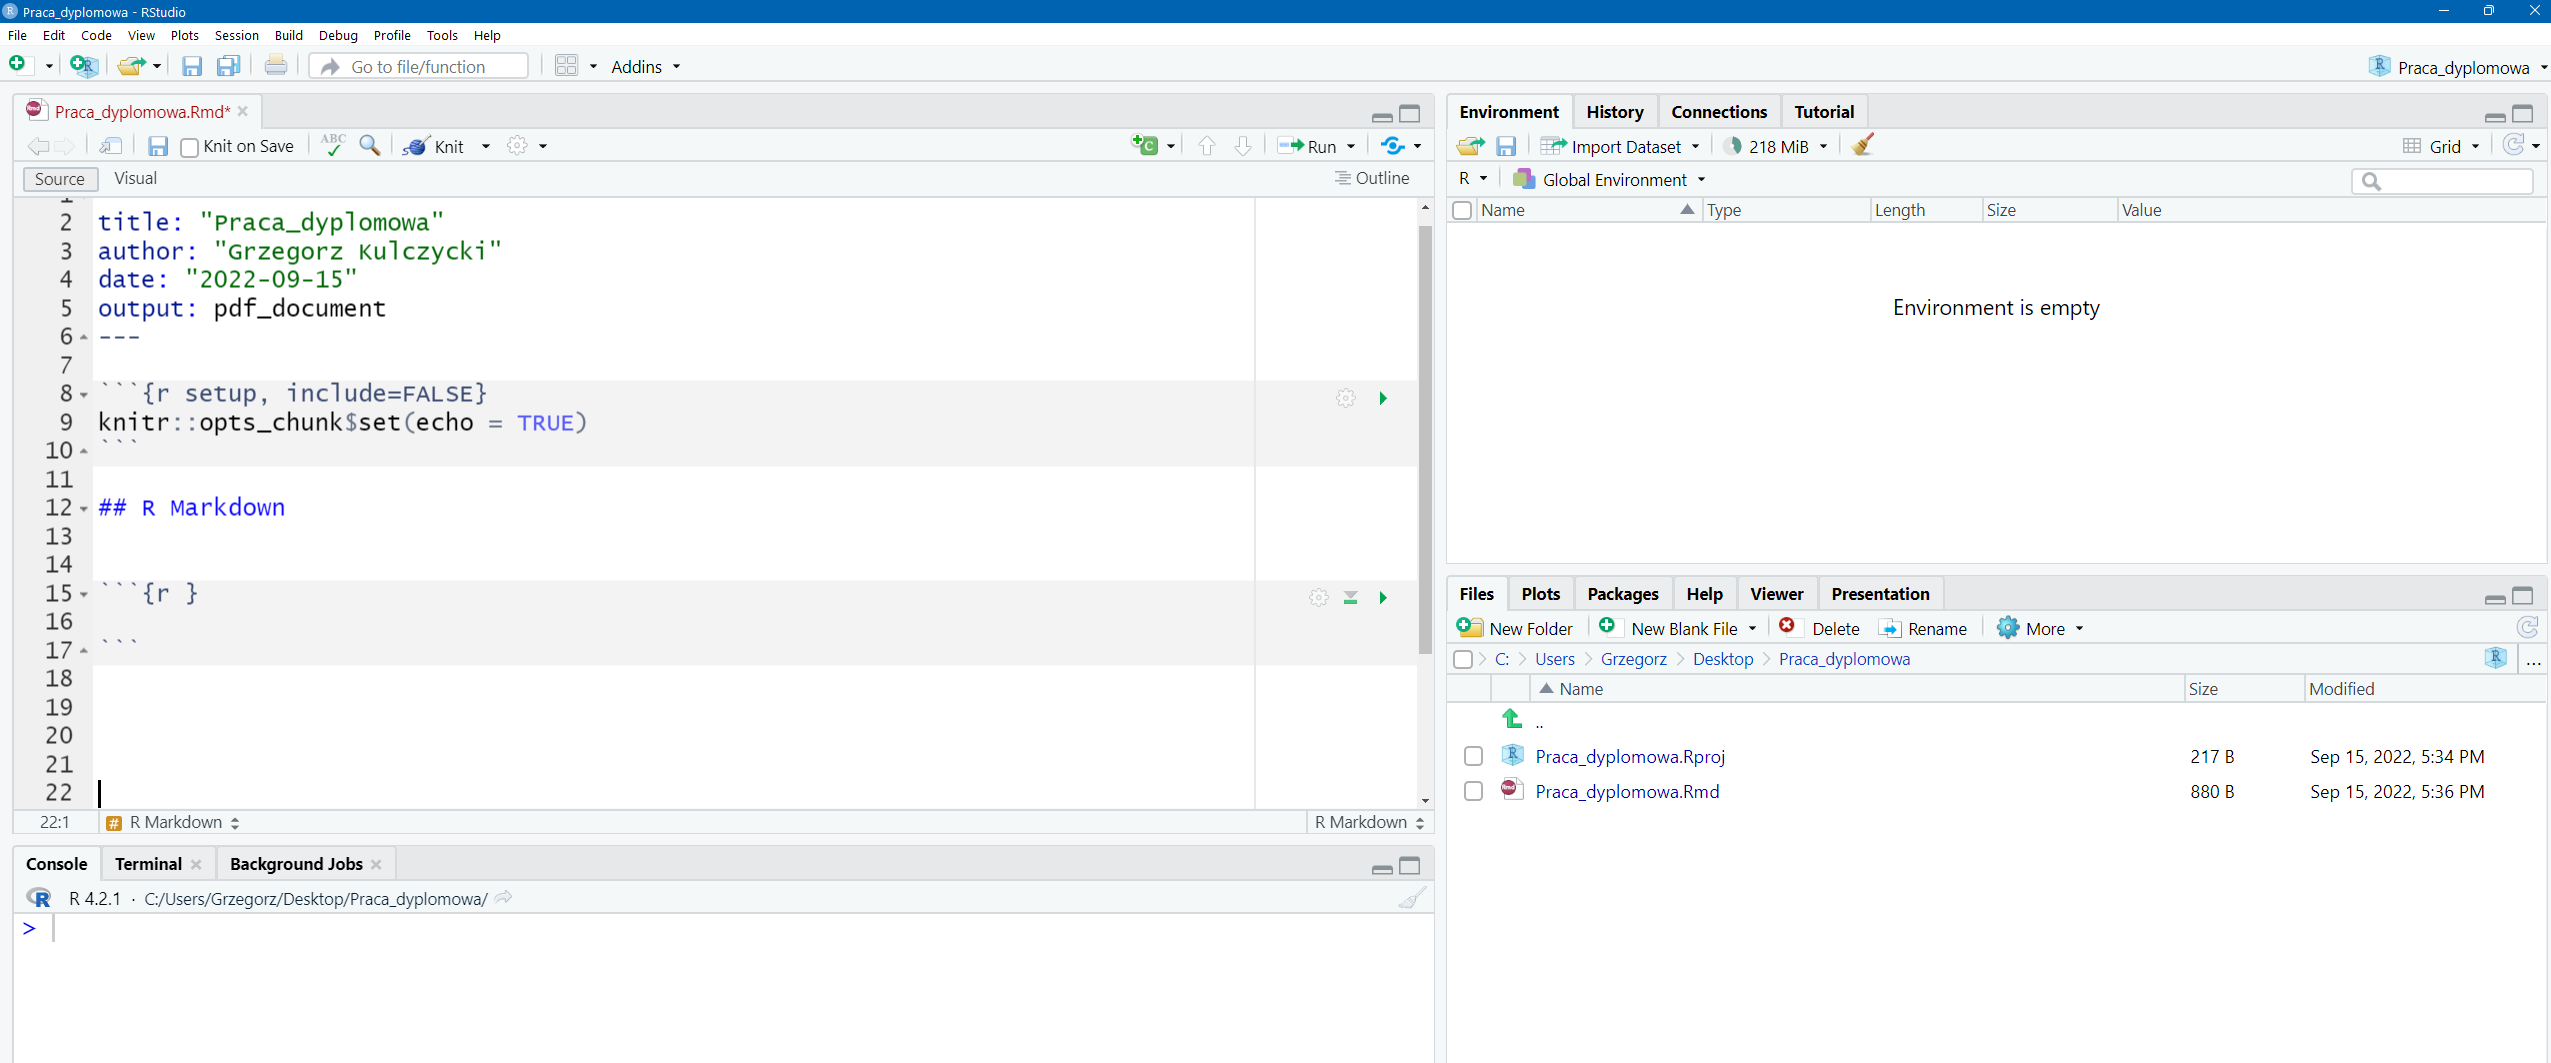
\includegraphics{Rysunki/nowy_projekt_rmd.png}
\caption{Plik .Rmd utworzony w ramach struktury projektu
\label{nowy_projekt_rmd}}
\end{figure}

\hypertarget{szablony-templatki-plikuxf3w-.rmd}{%
\subsubsection{Szablony (templatki) plików
.Rmd}\label{szablony-templatki-plikuxf3w-.rmd}}

Pliki \texttt{.Rmd} można tworzyć na domyślnych szablonach RStudio, bądź
na szablonach, które dostarczane są wraz z dedykowanymi bibliotekami.
Przykładowo pakiet rticles
(\protect\hyperlink{ref-allairexiedervieuxrfoundationwickhamjournalofstatisticalsoftwarevaidyanathanassociationforcomputingmachineryboettigerelsevierbromanmuellerquastpruimmarwickwickhamkeyesyuemaasitonkelinxgasparinidesautelsleutnantmdpitaylorandfrancisogredenhancenustuvestencampitellimuschellihayeskamvarrosscannoodtluguernkaplankreutzerwanghesselberthhyndman2022}{Allaire
i in., 2022}) dostarcza zestaw niestandardowych formatów R Markdown i
szablonów do tworzenia artykułów w czasopismach i zgłoszeń na
konferencje. Inne pakiety zawierające szablony artykułów naukowych to:
stevetemplates (\protect\hyperlink{ref-miller2021}{Miller, 2021}),
pagedown (\protect\hyperlink{ref-xielesurthornetan2022}{Xie i in.,
2022}), papaja (\protect\hyperlink{ref-austbarth2022}{Aust i Barth,
2022}), papeR (\protect\hyperlink{ref-hofner2021}{Hofner, 2021}), czy
thesisdown (\protect\hyperlink{ref-ismaysolomon2022}{Ismay i Solomon,
2022}).

\hypertarget{renderowanie-kompilowanie}{%
\subsection{Renderowanie
(kompilowanie)}\label{renderowanie-kompilowanie}}

Utworzone pliki \texttt{.Rmd} możemy edytować z wykorzystaniem języka
Markdown i osadzać w nich kody R.

Tworzenie dynamicznego dokumentu następuje w w procesie renderowania.
Proces ten polega na przedstawieniu informacji zapisanych w pliku w
określonej przez użytkownika formie (np. HTML, PDF, DOCX). Proces ten
możemy rozpocząć poprzez naciśniecie przycisku

\includegraphics{Rysunki/button_knit.png}.

W trakcie kompilacji (rys. \ref{konwersja_Rmd}) pakiet knitr jest
używany do przetworzenia wstawek kodu na czysty tekst w tymczasowym
dokumencie Markdown. Następnie względem tego pośredniego dokumentu
wywoływany jest program pandoc w celu przekonwertowania go na dokument
wyjściowy (\protect\hyperlink{ref-lander2018}{Lander, 2018}).

\begin{figure}
\centering
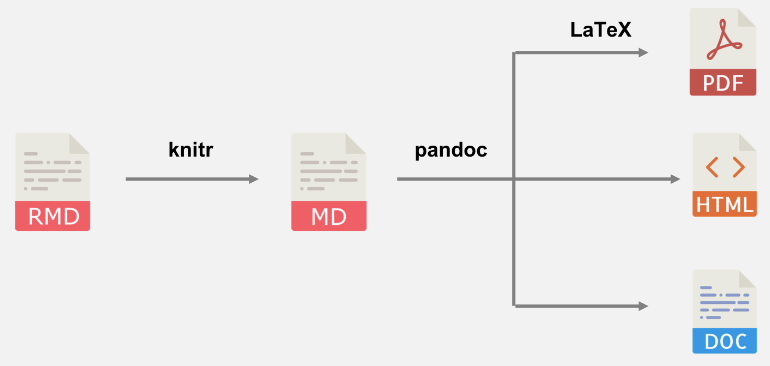
\includegraphics[width=0.7\textwidth,height=\textheight]{Rysunki/konwersja_Rmd.png}
\caption{Schemat konwersji dokumentu R Markdown \label{konwersja_Rmd}}
\end{figure}

Wynikiem renderowania są pliki o określonym wcześniej formacie który
został zapisany w ustawieniach (nagłówek YAML). Oficjalna strona
\href{https://rmarkdown.rstudio.com/index.html}{R Markdown} dla RStudio
podaje szereg możliwych plików wynikowych (output) rys.
\ref {output_Rmd} ).

\begin{figure}
\centering
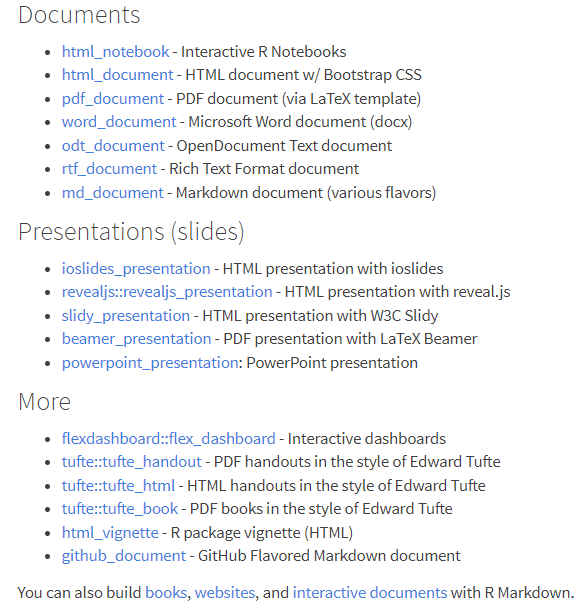
\includegraphics[width=0.58\textwidth,height=\textheight]{Rysunki/output_Rmd.png}
\caption{Możliwe do uzyskania pliki wynikowe w R Markdown
\label{output_Rmd}}
\end{figure}

\hypertarget{ustawienia-dokumentu-r-markdown}{%
\subsection{Ustawienia dokumentu R
Markdown}\label{ustawienia-dokumentu-r-markdown}}

\hypertarget{nagux142uxf3wek-yaml}{%
\subsubsection{Nagłówek YAML}\label{nagux142uxf3wek-yaml}}

Metadane YAML (zwane również nagłówkiem YAML) umieszczane są na samym
początku dokumentu zawierają szczegóły dotyczące całego dokumentu .
Nagłówek yaml (rys. \ref{naglowek_yaml}) jest wydzielany wierszami
zawierającymi po trzy dywizy przed i po nagłówku
(\protect\hyperlink{ref-lander2018}{Lander, 2018};
\protect\hyperlink{ref-xieallairegrolemund2018}{Xie i in., 2018}).

\begin{figure}
\centering
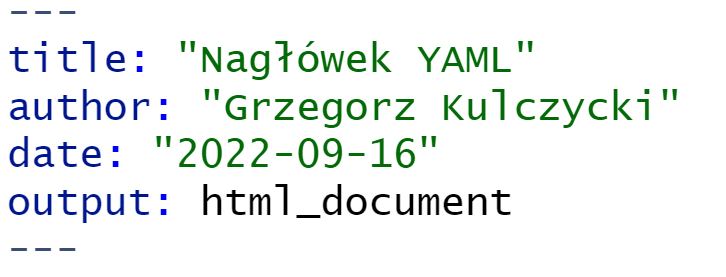
\includegraphics[width=0.35\textwidth,height=\textheight]{Rysunki/naglowek_yaml.png}
\caption{Przykład nagłówka yaml \label{naglowek_yaml}}
\end{figure}

Każdy wiersz nagłówka ma postać pary klucz-wartość, specyfikującej
argumenty dla dokumentu, takie jak title, author, date lub output (typ
dokumentu wyjściowego)(\protect\hyperlink{ref-lander2018}{Lander,
2018}).

Metadane YAML są bardzo wrażliwe na błędy dlatego warto zapoznać się z
dokumentacją dotyczącą ich użycia. Na stronie
\href{https://cran.r-project.org/web/packages/ymlthis/vignettes/yaml-overview.html}{CRAN}
(The Comprehensive R Archive Network) projektu R przedstawiona jest
podstawowa składnia YAML.

W nagłówku YAML można także zdefiniować tworzenie pliku tex
(rys.\ref{keep_tex}), który można edytować z użyciem edytorów LaTex.

\begin{figure}
\centering
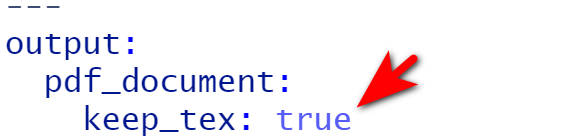
\includegraphics[width=0.37\textwidth,height=\textheight]{Rysunki/keep_tex.png}
\caption{Składnia do tworzenia pliku tex \label{keep_tex}}
\end{figure}

Wydawnictwa naukowe często preferują wykorzystanie LaTeX przy składzie
tekstu, gdyż wytworzenie tego pliku umożliwia szybkie nanoszenie
poprawek np. po recenzjach w procesie wydawniczym artykułu naukowego.

\hypertarget{skux142adnia-r-markdown}{%
\subsubsection{Składnia R Markdown}\label{skux142adnia-r-markdown}}

Markdown to język prostych znaczników, który powstał w celu uproszczenia
formatowania i przyspieszenia pracy nad dokumentami tekstowymi. Zaletą
składni R Markdown jest to, że dokumenty powstałe dzięki użyciu tego
języka są w pełni powtarzalne.

Na stronie \href{https://rmarkdown.rstudio.com/authoring_basics.html}{R
Markdown dla RStudio} zamieszczona jest podstawowa i najczęściej używana
składnia R Markdown.

W RStudio w panelu edycyjnym w zakładce Help → Cheat Sheets (rys.
\ref {help_rmarkdown} zamieszczone zostały odnośniki do materiałów
syntetycznie przedstawiających składnię R Markdown (rys.
\ref{cheat_rmarkdown}).

\begin{figure}
\centering
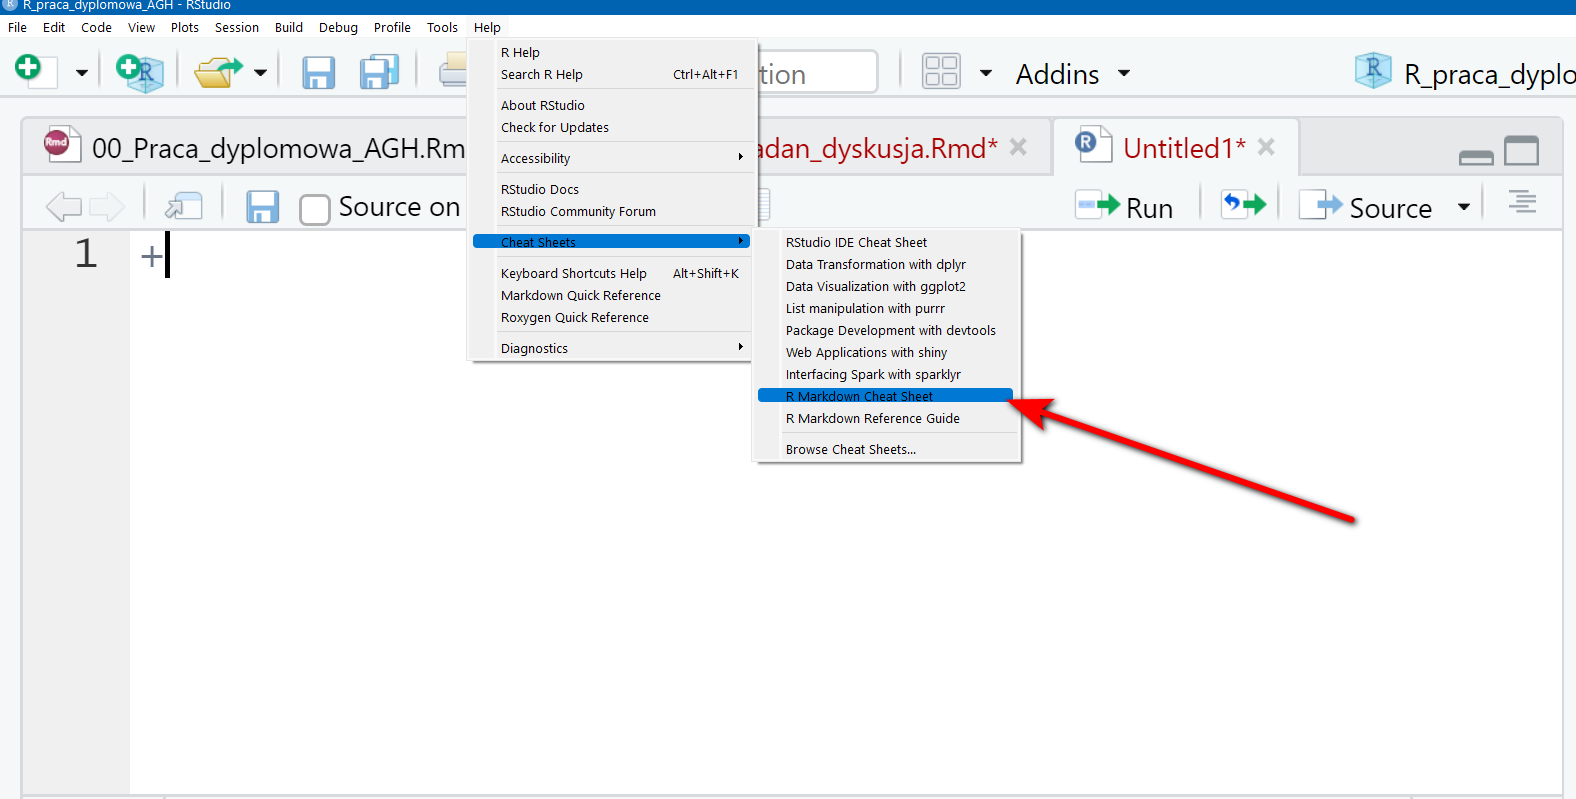
\includegraphics{Rysunki/help_rmarkdown.png}
\caption{Odnośnik do materiałów składni R Markdown
\label{help_rmarkdown}}
\end{figure}

\begin{figure}
\centering
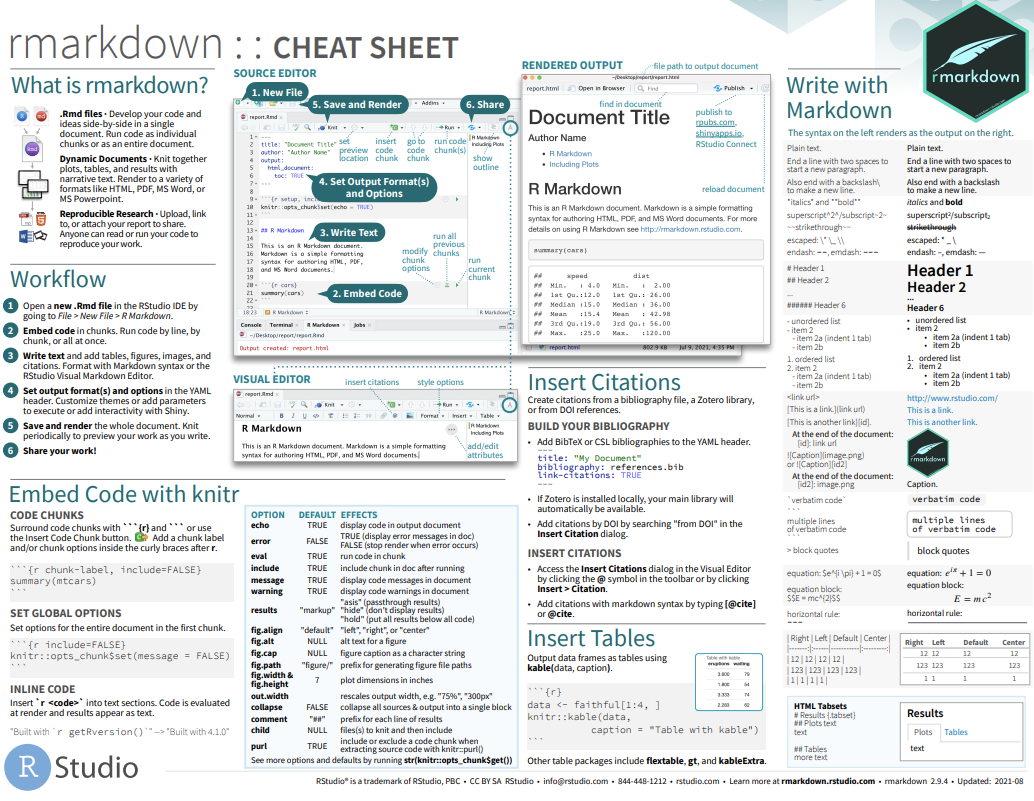
\includegraphics[width=1\textwidth,height=\textheight]{Rysunki/cheat_rmarkdown.png}
\caption{Syntetyczne materiały składni R Markdown
\label{cheat_rmarkdown}}
\end{figure}

\hypertarget{wstawki-kodu-w-markdown}{%
\subsubsection{Wstawki kodu w Markdown}\label{wstawki-kodu-w-markdown}}

W R Markdown istnieje możliwość osadzania kodów najważniejszych języków
programowania oraz baz danych np. R, Bash, D3, Python, Rcpp, SQL, Stan.

Osadzenie języków w R Markdown odbywa się z wykorzystaniem wstawki kodu
(chunks) (rys. \ref{wstawka_kodu}).

Początek wstawki jest oznaczany
\texttt{\textasciigrave{}\textasciigrave{}\textasciigrave{}\{r\}\ i\ kończy\ się\ znakami\textasciigrave{}\textasciigrave{}\textasciigrave{}},
kod wewnątrz wstawki traktowany jako kod w języku R
(\protect\hyperlink{ref-lander2018}{Lander, 2018}).

\begin{figure}
\centering
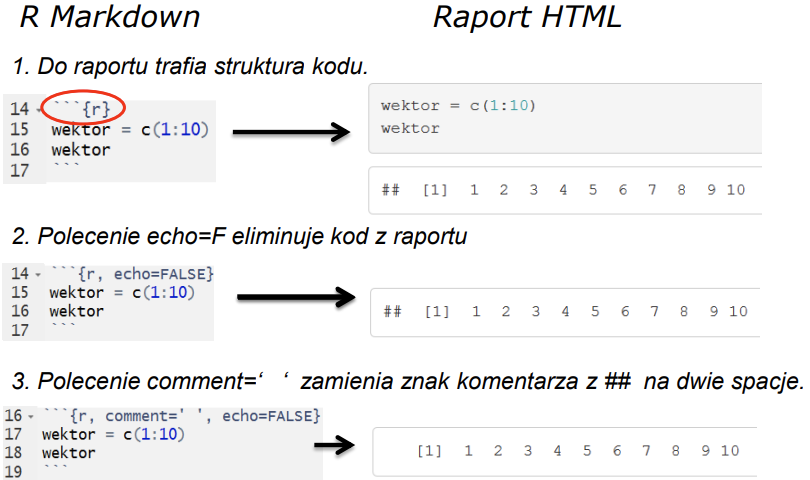
\includegraphics[width=0.6\textwidth,height=\textheight]{Rysunki/wstawka_kodu.png}
\caption{Osadzenie języków w R Markdown
(\protect\hyperlink{ref-strus2017}{Struś, 2017}). \label{wstawka_kodu}}
\end{figure}

\hypertarget{kod-r-w-linii-tekstu}{%
\subsubsection{Kod R w linii tekstu}\label{kod-r-w-linii-tekstu}}

Funkcjonalnym rozwiązaniem wstawiania kodu R jest także możliwość jego
umieszczania w linii tekstu (inline kod). Kod inline wyświetli wyniki,
ale nie ujawniając składni samego kodu (rys. \ref{inline_kod}).

\begin{figure}
\centering
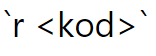
\includegraphics[width=0.1\textwidth,height=\textheight]{Rysunki/inline_kod.png}
\caption{Struktura kodu R w linii tekstu\label{inline_kod}}
\end{figure}

\hypertarget{cytowanie-literatury-w-r-markdown}{%
\subsection{Cytowanie literatury w R
Markdown}\label{cytowanie-literatury-w-r-markdown}}

Pisanie publikacji naukowych nierozerwalnie związane jest z cytowaniami
prac innych autorów, którzy wykonywali podobne badania.

W celu identyfikacji publikacji naukowej i odróżnienia jej od innych
wykorzystuje się opis bibliograficzny, czyli uporządkowany zespół danych
cech dokumentu. Opis bibliograficzny publikacji zamieszczony na stronach
wydawnictw naukowych może być dostępny w rożnych formatach w zależności
od menadżera bibliografii. Obecnie dostępnych jest dla użytkownika kilka
menadżerów publikacji zarówno komercyjnych, jak i darmowych. Najbardziej
popularne to Citavi, Mendeley, EndNote, Zotero, RefWorks i Papers.

W pracy z plikami R Markdown zalecanym menadżerem cytowań jest
\href{https://www.zotero.org/}{Zotero}. Dobrym rozwiązaniem podczas
pracy z tym menadżerem jest wykorzystanie dodatku (plugin)
\href{https://retorque.re/zotero-better-bibtex/}{Better BibTeX (BBT)},
który automatycznie generuje klucze cytatów.

Większość wydawnictw umożliwia pobranie cytowania danej publikacji w
formacie BibTeX (rys. \ref{format_bibtex}) lub pobranie cytowania przez
dodatki do przeglądarek np.
\href{https://chrome.google.com/webstore/detail/zotero-connector/ekhagklcjbdpajgpjgmbionohlpdbjgc?hl=pl}{Zotero
Connector} dla przegladarki Chrome.

\begin{figure}
\centering
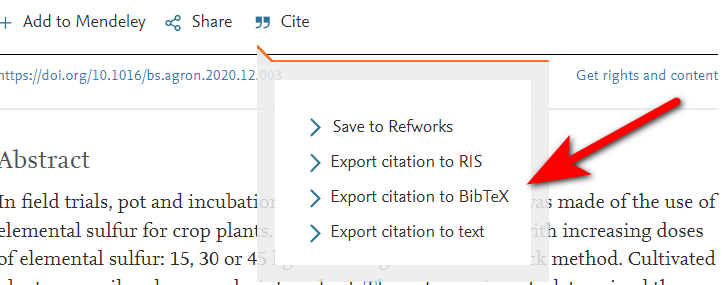
\includegraphics[width=0.8\textwidth,height=\textheight]{Rysunki/format_bibtex.png}
\caption{Pobieranie cytowania ze strony ELSEVIER \label{format_bibtex}}
\end{figure}

\hypertarget{wspuxf3ux142praca-zotero-w-rstudio}{%
\subsubsection{Współpraca Zotero w
RStudio}\label{wspuxf3ux142praca-zotero-w-rstudio}}

Pracując z plikami \texttt{.Rmd} istnieje możliwość edycji pliku w
trybie skryptowym (Source) oraz wizualnego edytora (Visual) (rys.
\ref{tryb_visual}).

\begin{figure}
\centering
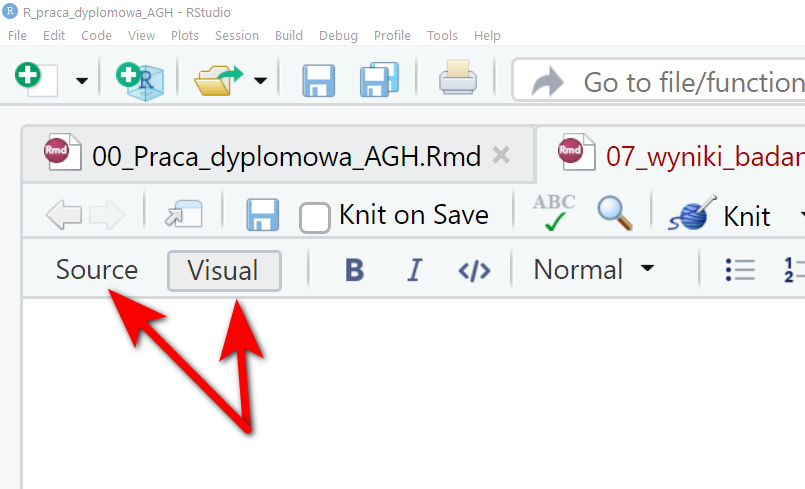
\includegraphics[width=0.5\textwidth,height=\textheight]{Rysunki/tryb_visual.png}
\caption{Przyciski zmiany trybu pracy edytora \label{tryb_visual}}
\end{figure}

W domyślnych ustawieniach RStudio: Tools→ Global Options→R Markdown →
Citations wstawienie cytowania odbywa się w trybie pracy z wizualnym
edytorem z wykorzystaniem menadżera publikacji Zotero (rys.
\ref{zotero_ustawienia}). Korzystając w Zotero z rozszerzenia Better
BibTex można także wybrać opcję korzystania z klucza cytowań
generowanego przez ten dodatek.

\begin{figure}
\centering
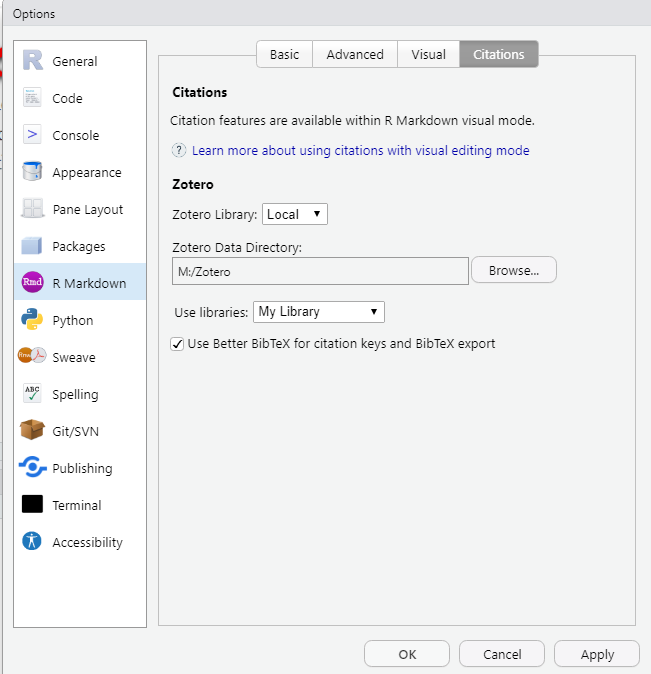
\includegraphics[width=0.6\textwidth,height=\textheight]{Rysunki/zotero_ustawienia.png}
\caption{Ustawienie wstawiania cytowań \label{zotero_ustawienia}}
\end{figure}

W trybie pracy skryptowym, żeby wstawiać cytowania trzeba zainstalować
określone biblioteki. Aktualnie jest możliwość skorzystania z pakietów
rbbt (\protect\hyperlink{ref-dunningtonwiernik2022}{Dunnington i
Wiernik, 2022}) oraz citr (\protect\hyperlink{ref-aust2019}{Aust,
2019}). Oba te pakiety obecnie nie są umieszczone w dokumentacji CRAN,
dlatego instalacja ich odbywa się z wykorzystaniem
\href{https://github.com/}{GitHub}.

Polecenia do instalacji pakietów do cytowania i ich uruchamiania
wyszczególniono na rys. \ref{cytowanie_pakiety}.

\begin{figure}
\centering
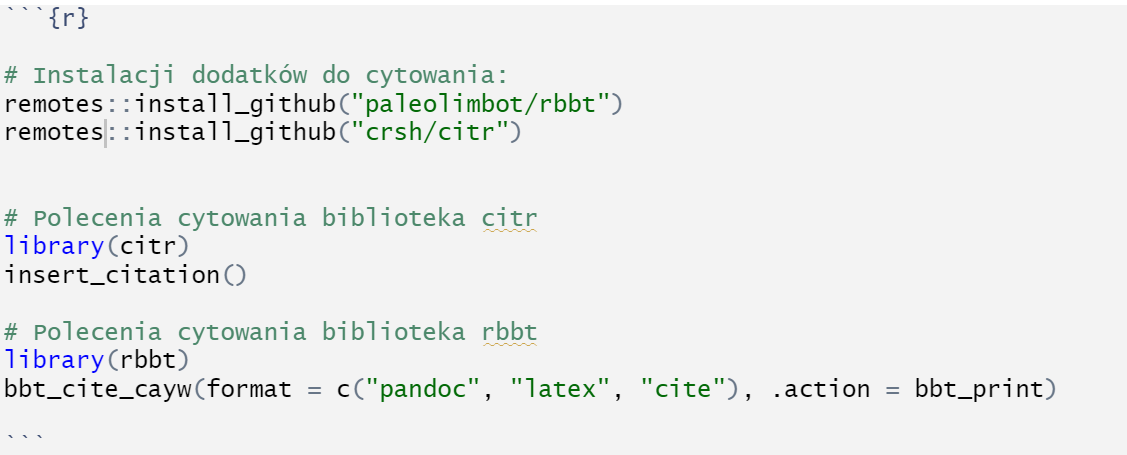
\includegraphics{Rysunki/cytowanie_pakiety.png}
\caption{Kod do uruchomienia pakietów do cytowania
\label{cytowanie_pakiety}}
\end{figure}

Wygodniejszą opcją jest zdefiniowanie dla tych dodatków skrótów
klawiszowych poprzez Tools → Modify Keyboard Shortcut (rys.
\ref{Keyboard_Shortcut}).

\begin{figure}
\centering
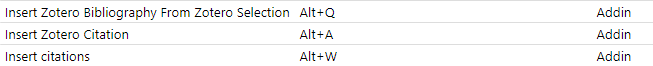
\includegraphics{Rysunki/Keyboard_Shortcut.png}
\caption{Definiowanie skrótów klawiszowych do cytowania
\label{Keyboard_Shortcut}}
\end{figure}

\hypertarget{definiowanie-opcji-bibliograficznych-w-pliku-.rmd}{%
\subsubsection{Definiowanie opcji bibliograficznych w pliku
.Rmd}\label{definiowanie-opcji-bibliograficznych-w-pliku-.rmd}}

W nagłówku YAML metadanych wymagane jest wskazanie ścieżki do pliku
bibliograficznego i miejsca jego umieszczenia. Poniżej umieszczono
przykładowe wskazanie pliku bibliograficznego (rys. \ref{bib_plik}),
czyli pliku tekstowego z rozszerzeniem \texttt{.bib}, w którym
zamieszczane są wpisy bibliograficzne w formie BiBTex (rys.
\ref{BibTex}):

\begin{figure}
\centering
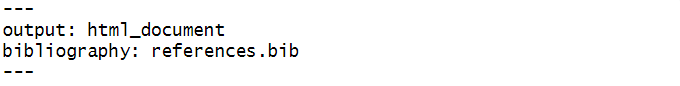
\includegraphics[width=0.8\textwidth,height=\textheight]{Rysunki/bib_plik.png}
\caption{Wskazanie ścieżki pliku bibliograficznego \label{bib_plik}}
\end{figure}

\begin{figure}
\centering
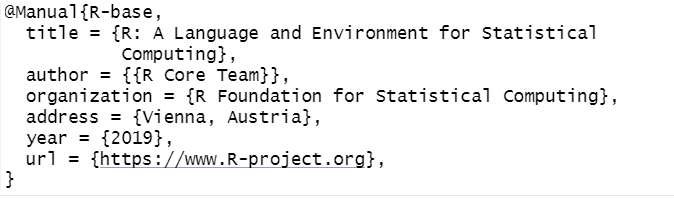
\includegraphics[width=0.75\textwidth,height=\textheight]{Rysunki/BibTex.png}
\caption{Wpis bibliograficzny w formie BiBTex \label{BibTex}}
\end{figure}

W nagłówku YAML metadanych można także określić styl cytowania, czyli
wstawić ścieżki do pliku z rozszerzeniem \texttt{.csl}. Domyślnie Pandoc
używa formatu Chicago author-date dla cytatów i spisu literatury. Aby
użyć innego stylu, należy podać plik CSL (Citation Style Language) w
polu metadanych (\protect\hyperlink{ref-xie2021}{Xie i in., 2021}).

\hypertarget{skux142adnia-cytowania}{%
\subsubsection{Składnia cytowania}\label{skux142adnia-cytowania}}

Składnia cytowania służy do odwoływania się do dokumentów i opiera się
na kluczach cytatów, a podstawowym blokiem konstrukcyjnym jest
@citationkey (rys. \ref{skladnia}).

\begin{figure}
\centering
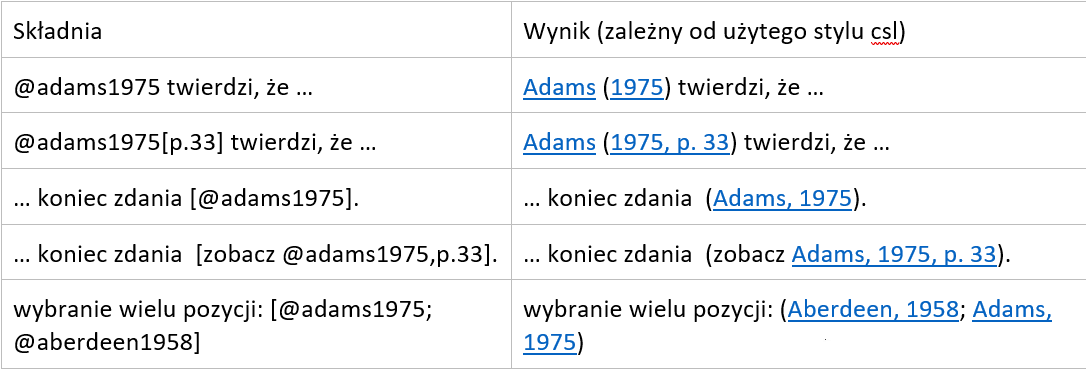
\includegraphics[width=0.8\textwidth,height=\textheight]{Rysunki/skladnia.png}
\caption{Składnia cytowań \label{skladnia}}
\end{figure}

\hypertarget{zamieszczenie-spisu-literatury}{%
\subsubsection{Zamieszczenie spisu
literatury}\label{zamieszczenie-spisu-literatury}}

Domyślnie, bibliografia umieszczona jest na końcu dokumentu. Spis
literatury można zamieścić w innym miejscu poprzez użycie składni jak na
rysunku \ref{spis_literatury}.

\begin{figure}
\centering
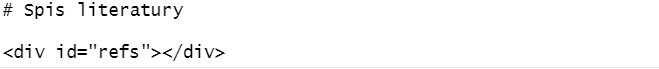
\includegraphics[width=0.6\textwidth,height=\textheight]{Rysunki/spis_literatury.png}
\caption{Określenie miejsca dla spisu literatury
\label{spis_literatury}}
\end{figure}

\hypertarget{studium-przypadku-case-study}{%
\subsection{Studium przypadku (case
study)}\label{studium-przypadku-case-study}}

Praktyczne wykorzystanie omawianych powyżej narzędzi umożliwiających
stworzenie publikacji naukowej w R Markdown w środowisku RStudio
zostanie omówione na przykładzie przyjętej do druku publikacji

Publikacja została stworzona z wykorzystaniem szablonu dla wydawnictwa
MDPI z pakietu rticles. Sekcja YAML dla szablonu MDPI (rys.
\ref{rticles_MDPI}) zawiera także odwołanie do formatowania w LaTeX,
dzięki czemu można opcjonalnie używać LaTeXa do tworzenia rysunków i
tabel.

\begin{figure}
\centering
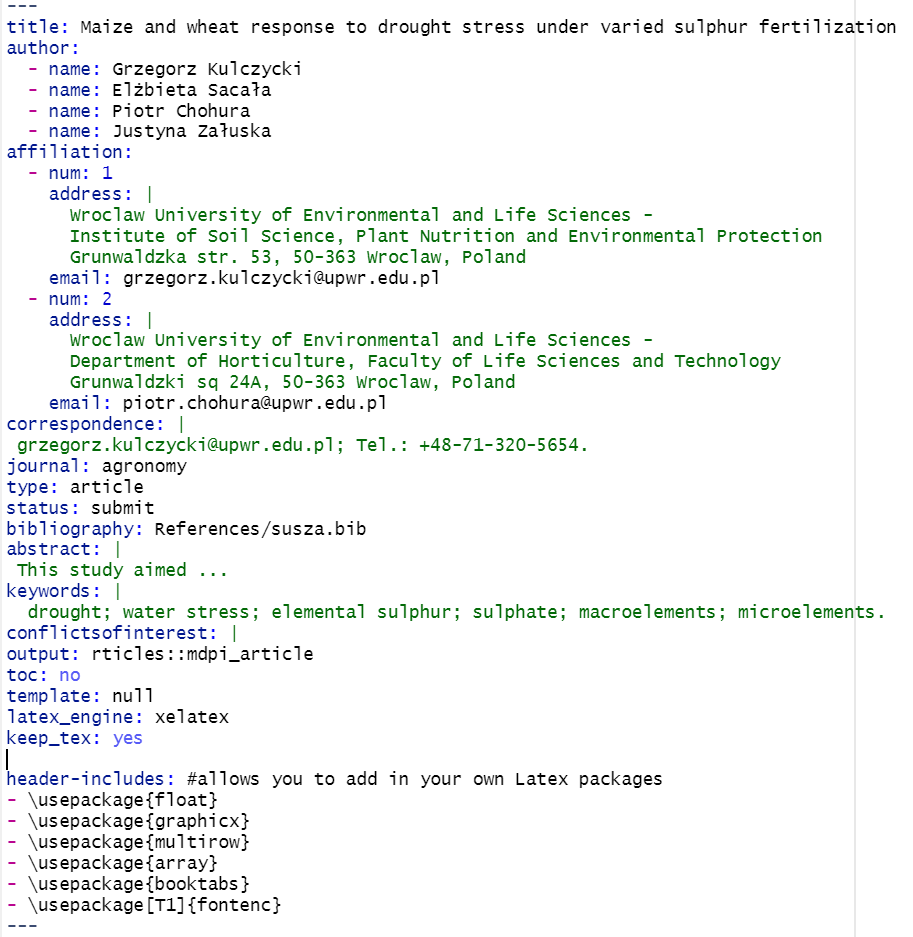
\includegraphics[width=0.8\textwidth,height=\textheight]{Rysunki/rticles_MDPI.png}
\caption{Sekcja YAML szablon MDPI \label{rticles_MDPI}}
\end{figure}

Wszystkie analizy statystyczne zostały wykonane w pliku \texttt{.R},
natomiast w pliku szablonu \texttt{.Rmd} umieszczono odwołanie we
wstawce kodu do tego pliku (rys. \ref{odwolanie_do_R}).

\begin{figure}
\centering
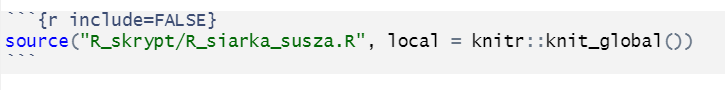
\includegraphics[width=0.7\textwidth,height=\textheight]{Rysunki/odwolanie_do_R.png}
\caption{Wstawka kodu z odwołaniem do pliku R \label{odwolanie_do_R}}
\end{figure}

W szablonie w poszczególnych rozdziałach umieszczano tekst publikacji,
natomiast we wstawkach kodu R odnośniki do tabel oraz rysunków.

Przykład wstawki kodu dla rysunku 4 w publikacji (rys. \ref{rysunek_4}
wraz z wynikiem (output) w publikacji (rys. \ref{figura_4}\}.

\begin{figure}
\centering
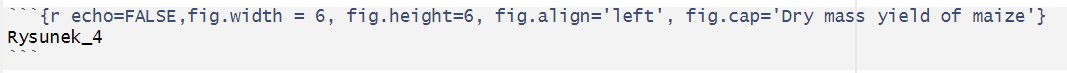
\includegraphics{Rysunki/rysunek_4.png}
\caption{Wstawka kodu z odwołaniem do rysunku 4 \label{rysunek_4}}
\end{figure}

\begin{figure}
\centering
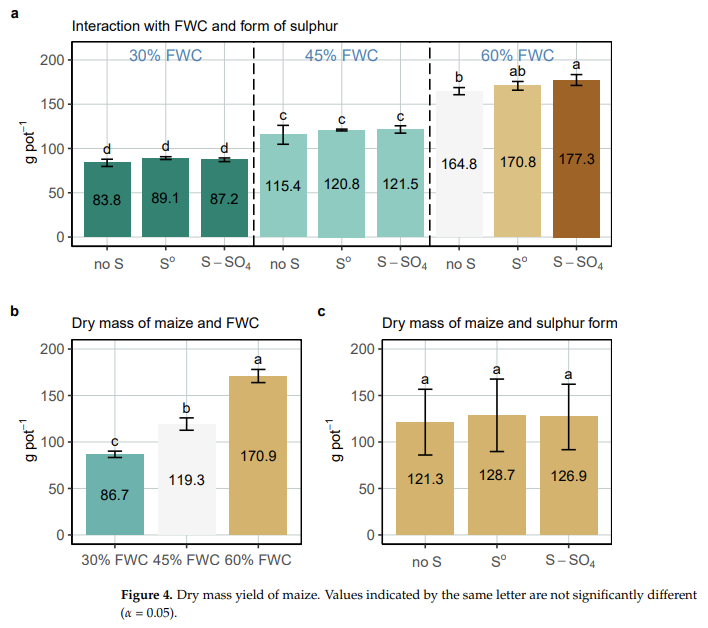
\includegraphics[width=0.8\textwidth,height=\textheight]{Rysunki/figura_4.png}
\caption{Przykład powtarzalności wykonania rysunku 4 w publikacji
\label{figura_4}}
\end{figure}

Wszystkie cytowania w artykule wykonano poprzez wstawianie @citationkey
z programu Zotero (rys. \ref{cytowania}).

\begin{figure}
\centering
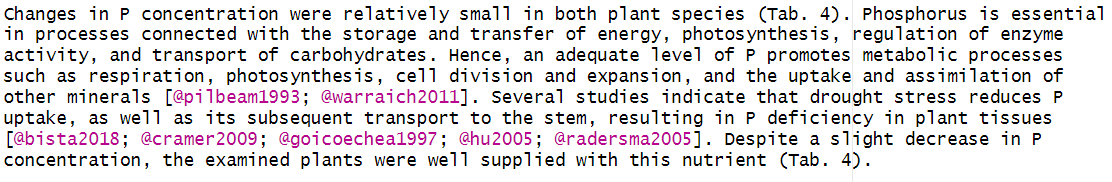
\includegraphics{Rysunki/cytowania.png}
\caption{Cytowania umieszczone w artykule \label{cytowania}}
\end{figure}

Po procesie renderowania otrzymano artykuł (rys. \ref{artykul}) zgodny z
wymaganiami wydawnictwa za pomocą zautomatyzowanego procesu jego
wytwarzania.

\begin{figure}
\centering
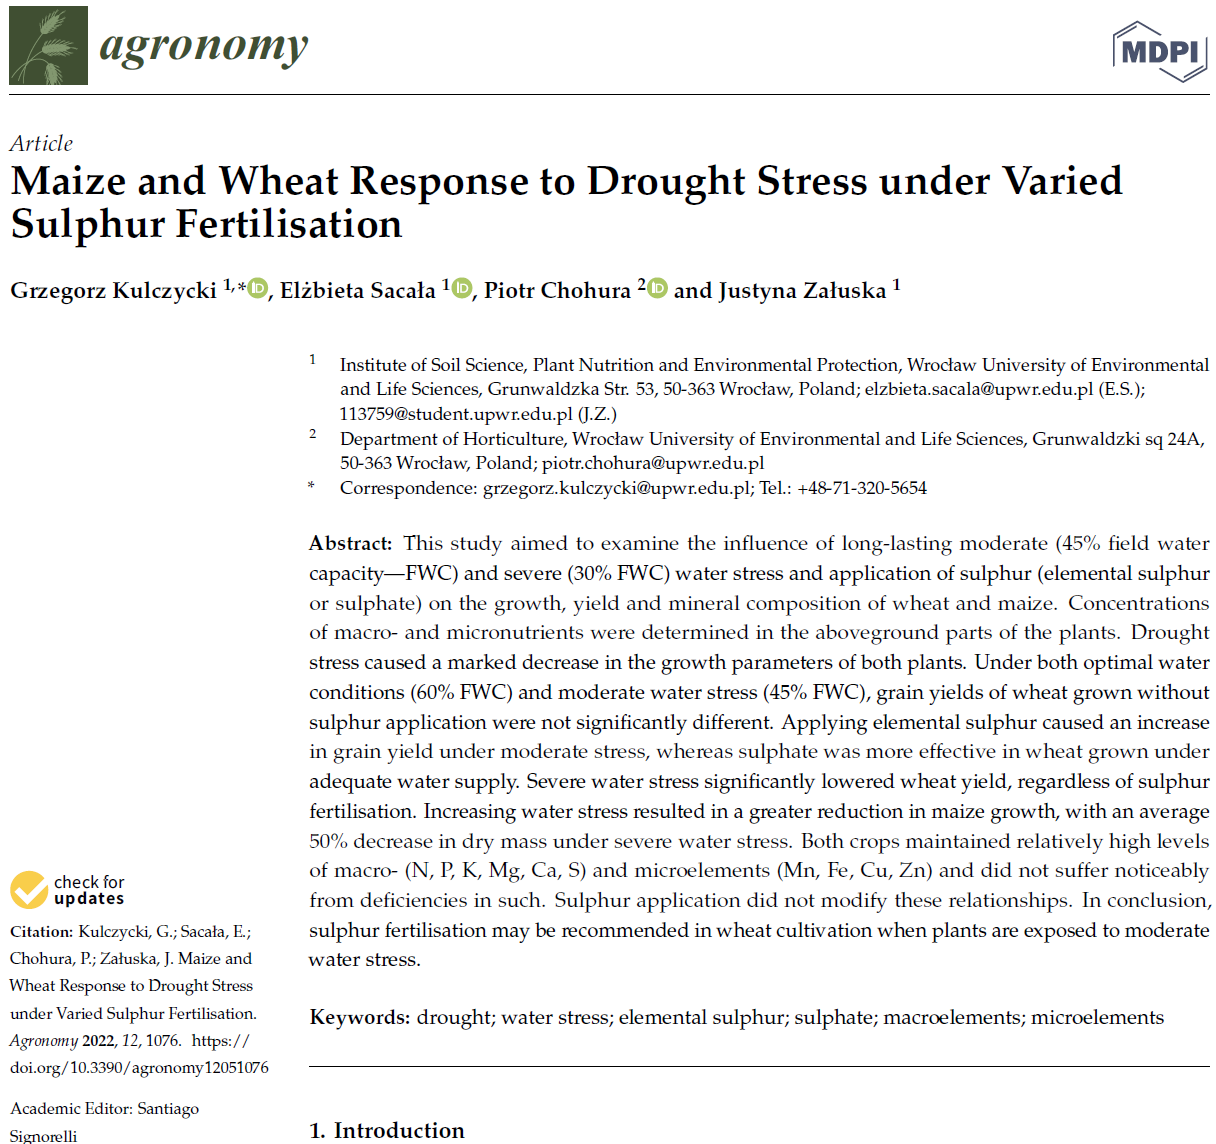
\includegraphics[width=0.8\textwidth,height=\textheight]{Rysunki/artykul.png}
\caption{Artykuł po procesie renderowania \label{artykul}}
\end{figure}

\hypertarget{dyskusja-wynikuxf3w}{%
\subsection{Dyskusja wyników}\label{dyskusja-wynikuxf3w}}

Fomel i Claerbout (\protect\hyperlink{ref-fomelclaerbout2009}{2009})
zaproponowali pojęcie powtarzalności badań określając, że produktem
końcowym badań jest nie tylko sama praca, ale także pełne środowisko
obliczeniowe użyte do wytworzenia końcowych wyników, takich jak kod i
dane niezbędne do odtworzenia wyników
(\protect\hyperlink{ref-xie2015}{Xie, 2015}).

Schemat ideowy badań naukowych z ich końcowym etapem w postaci napisania
publikacji przedstawiono na rysunku \ref{schemat_odtwarzania}
(modyfikacja własna za (\protect\hyperlink{ref-pebesma2016}{Pebesma,
2016})).

\begin{figure}
\centering
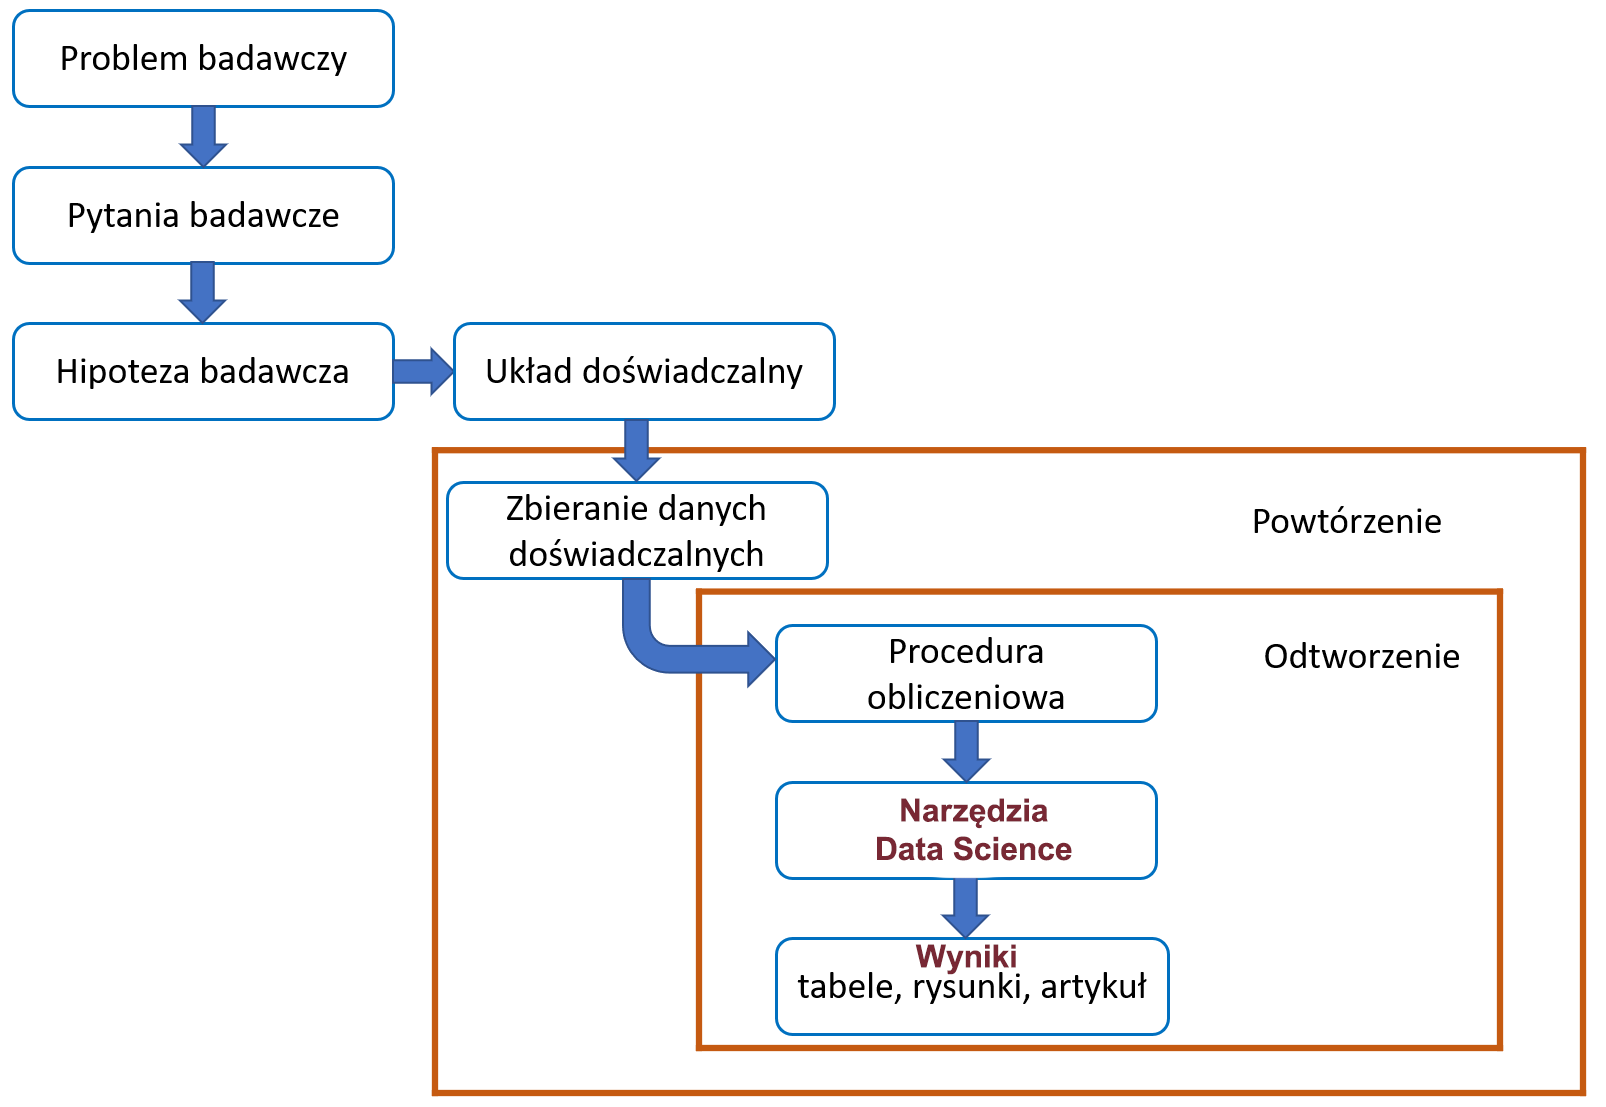
\includegraphics[width=0.9\textwidth,height=\textheight]{Rysunki/schemat_odtwarzania.png}
\caption{Schemat ideowy badań naukowych \label{schemat_odtwarzania}}
\end{figure}

Zaletą użycia metod odtwarzalnych wyników jest także zdolność do
powtórzenia obliczeń z dokładnie takim samym wynikiem jak pierwotnie
otrzymane, czyli wysoka powtarzalność (reproducibility).

O wysokiej odtwarzalności wyników badań mówi się wtedy gdy uzyskane
wyniki z eksperymentu lub w analizie statystycznej z zestawu danych są
ponownie osiągnięte z wysokim stopniem powtarzalności, gdy badania są
replikowane.

King (\protect\hyperlink{ref-king1995}{1995}) stwierdza, że wyniki badań
są powtarzalne, jeśli dostępne są wystarczające informacje, aby
niezależni badacze mogli dokonać tych samych ustaleń przy użyciu tych
samych procedur.

Zakłada się, że skuteczne dostarczenie wyników analizy może być równie
istotne, jak sama analiza, dlatego ważne jest żeby otrzymywać rezultaty
pracy w efektywny sposób (\protect\hyperlink{ref-lander2018}{Lander,
2018}).

Peng (\protect\hyperlink{ref-peng2016a}{2016}) wskazuje na elementy
odtwarzalności które są wymagane, aby wyniki były powtarzalne:

\begin{itemize}
\item
  dane analityczne dostępne dla innych, będące kluczowe do wykonania
  analizy danych.
\item
  kod analityczny użyty do uzyskania wyników z danych analitycznych.
\item
  dokumentacja kodu i danych
\item
  dystrybucja tak aby wszystkie dane w kodzie były łatwo dostępne.
\end{itemize}

Korzyścią zastosowania odtwarzalnych metod jest możliwość skupienia się
na pisaniu pracy bez konieczności zajmowania się edycyjnymi
zagadnieniami jak podziały na strony, układ strony, czcionki, numeracje
rysunków czy tabel.

Użycie narzędzi do badań odtwarzalnych stwarza możliwości wydajniejszej
pracy, a po nabraniu doświadczenia i umiejętności w użyciu tych narzędzi
praca możne się okazać szybsza i łatwiejsza do wykonania.

Do zalet korzystania z metody powtarzalnych badań można także zaliczyć
(\protect\hyperlink{ref-brookerachelnicholas2022}{Brooke i in., 2022}):

\begin{itemize}
\item
  szybką orientację w wykonanej pracy po upływie dłuższego czasu od jej
  ukończenia,
\item
  łatwość wprowadzenia poprawek do kodu lub danych, nawet na wczesnym
  etapie procesu, i ponowne przeprowadzenie całej analizy,
\item
  możliwość podzielenia się swoją pracą z innymi wykorzystując np.
  GitHub.
\end{itemize}

Zaletą pisania powtarzalnych dokumentów w R Markdown jest to, że mamy
możliwość dostarczyć tę samą informację w wielu formatach wyjściowych
np. PDF, DOCX, HTML (\protect\hyperlink{ref-racine2017}{Racine, 2017}).

Oczywiście, należy mieć świadomość barier które mogą wystąpić w okresie
poznawania narzędzi badawczych. Bariery te związane są głównie z
dodatkowym nakładem pracy, gdyż przyjmuje się, że początkowy nakład
pracy jest duży w porównaniu do osiąganych efektów. Jednak trend ten po
pewnym czasie ulega odwróceniu i nakład pracy, który został poniesiony
na początku w dalszej perspektywie przynosi duży wzrost efektywności
pracy (rys. \ref{r_first_then})

\begin{figure}
\centering

\includegraphics[width=0.65\textwidth,height=\textheight]{Rysunki/r_first_then.png}
\caption{Zmiana nastawienia do programu R (rysunek wykonała
\href{https://github.com/allisonhorst/stats-illustrations/}{Allison
Horst}) \label{r_first_then}}
\end{figure}

\FloatBarrier
\newpage
\fancyhead[C]{Wnioski}

\hypertarget{wnioski}{%
\section{Wnioski}\label{wnioski}}

\textbf{Na podstawie przeprowadzonych badań wyciągnięto następujące
wnioski:}

\begin{enumerate}
\def\labelenumi{\arabic{enumi}.}
\item
  Środowisko pracy programu R z jego graficznym interfejsem RStudio oraz
  biblioteką R Markdown umożliwia przeprowadzenie tworzenia publikacji
  naukowych w pełni powtarzalnych (rys. \ref{reproducibility_court}).
\item
  R Markdown tworzy dynamiczne dokumenty poprzez możliwość zastosowania
  zagnieżdżonych kodów języków programowania.
\item
  Zastosowanie powtarzalnych metod publikowania pozwala na
  zautomatyzowanie tego procesu przyczyniając się do zwiększenia
  efektywności pracy naukowej.
\item
  Konwersja wyników pracy do różnych formatów stanowi istotną zaletę
  korzystania z tych narzędzi pracy w porównaniu do tradycyjnych metod
  korzystania z popularnych edytorów tekstu.
\item
  Zaletą korzystania z odtwarzalnych metod jest możliwość skupienia się
  na pisaniu pracy bez konieczności zajmowania się problemami edycyjnymi
  przy tworzeniu dokumentu.
\item
  Wymagany początkowy duży nakład pracy w opanowanie środowiska pracy R,
  możne wpływać zniechęcająco na potencjalnych użytkowników tego
  oprogramowania, ale w dłuższej perspektywie zdecydowanie zwiększa
  efektywność pracy przy tworzeniu publikacji naukowych.
\end{enumerate}

\begin{figure}
\centering

\includegraphics[width=0.5\textwidth,height=\textheight]{Rysunki/reproducibility_court.png}
\caption{Potwierdzenie powtarzalności dokumentu (rysunek wykonała
\href{https://github.com/allisonhorst/stats-illustrations/}{Allison
Horst}) \label{reproducibility_court}}
\end{figure}

\FloatBarrier
\newpage
\fancyhead[C]{Literatura}

\hypertarget{literatura}{%
\section{Literatura}\label{literatura}}

\hypertarget{refs}{}
\begin{CSLReferences}{1}{0}
\leavevmode\vadjust pre{\hypertarget{ref-allairexiedervieuxrfoundationwickhamjournalofstatisticalsoftwarevaidyanathanassociationforcomputingmachineryboettigerelsevierbromanmuellerquastpruimmarwickwickhamkeyesyuemaasitonkelinxgasparinidesautelsleutnantmdpitaylorandfrancisogredenhancenustuvestencampitellimuschellihayeskamvarrosscannoodtluguernkaplankreutzerwanghesselberthhyndman2022}{}}%
Allaire, J., Y. Xie, C. Dervieux, R Foundation, H. Wickham, i in. 2022.
Rticles: {Article} Formats for {R} Markdown.

\leavevmode\vadjust pre{\hypertarget{ref-apanowicz2005}{}}%
Apanowicz, J. 2005. Metodologiczne uwarunkowania pracy naukowej. Prace
doktorskie. Prace habilitacyjne. Difin, Warszawa.

\leavevmode\vadjust pre{\hypertarget{ref-aust2019}{}}%
Aust, F. 2019. Citr: '{RStudio}' Add-in to Insert Markdown Citations.

\leavevmode\vadjust pre{\hypertarget{ref-austbarth2022}{}}%
Aust, F., i M. Barth. 2022. Papaja: {Prepare} Reproducible {APA} Journal
Articles with {R Markdown}.

\leavevmode\vadjust pre{\hypertarget{ref-biecek2017}{}}%
Biecek, P. 2017. Przewodnik po pakiecie R. Oficyna Wydawnicza GiS,
Wroc{ł}aw.

\leavevmode\vadjust pre{\hypertarget{ref-borkowski2015}{}}%
Borkowski, M., i B. Przybylski. 2015. LATEX ksi{ą}{ż}ka kucharska.
Polskie Towarzystwo Matematyczne.

\leavevmode\vadjust pre{\hypertarget{ref-brookerachelnicholas2022}{}}%
Brooke, A., S. Rachel, i G. Nicholas. 2022. R {Programming} for
{Research}. {Colorado State University, ERHS 535}.

\leavevmode\vadjust pre{\hypertarget{ref-comarch2023}{}}%
Comarch. 2023. Ranking najpopularniejszych języków programowania według
TIOBE Index.
\url{https://kariera.comarch.pl/blog/python-na-czele-julia-pierwszy-raz-w-czolowej-dwudziestce-ranking-najpopularniejszych-jezykow-programowania-wedlug-tiobe-index/}.

\leavevmode\vadjust pre{\hypertarget{ref-cooper1986}{}}%
Cooper, H.M. 1986. The integrative research review: a systematic
approach. 2. print. Sage.

\leavevmode\vadjust pre{\hypertarget{ref-creswell2013}{}}%
Creswell, J.W. 2013. Projektowanie badań naukowych Metody jakościowe,
ilościowe i mieszane. Wydawnictwo Uniwersytetu Jagiellońskiego.

\leavevmode\vadjust pre{\hypertarget{ref-curcic2023}{}}%
Curcic, D. 2023. Number of academic papers published per year.
WordsRated.

\leavevmode\vadjust pre{\hypertarget{ref-dunningtonwiernik2022}{}}%
Dunnington, D., i B.M. Wiernik. 2022. Rbbt: {R} Interface to the Better
{BiBTex} Zotero Connector.

\leavevmode\vadjust pre{\hypertarget{ref-dz.u.2019}{}}%
Dz. U. 2019. Rozporz{ą}dzenie Ministra Nauki i Szkolnictwa Wy{ż}szego z
dnia 22 lutego 2019 r. w sprawie ewaluacji jako{ś}ci dzia{ł}alno{ś}ci
naukowej Poz. 392.

\leavevmode\vadjust pre{\hypertarget{ref-fomelclaerbout2009}{}}%
Fomel, S., i J. Claerbout. 2009. Guest Editors' Introduction:
{Reproducible} Research. Computing in Science \& Engineering 11(1):
5--7.

\leavevmode\vadjust pre{\hypertarget{ref-guxf3recki2011}{}}%
Górecki, T. 2011. Podstawy statystyki z przyk{ł}adami w R. Wydawnictwo
BTC, Legionowo.

\leavevmode\vadjust pre{\hypertarget{ref-hofner2021}{}}%
Hofner, B. 2021. {papeR}: {A} Toolbox for Writing Pretty Papers and
Reports.

\leavevmode\vadjust pre{\hypertarget{ref-ismaysolomon2022}{}}%
Ismay, C., i N. Solomon. 2022. Thesisdown: {An} Updated {R Markdown}
Thesis Template Using the Bookdown Package.

\leavevmode\vadjust pre{\hypertarget{ref-king1995}{}}%
King, G. 1995. Replication, {Replication}. PS: Political Science and
Politics 28(3): 444. doi:
\href{https://doi.org/10.2307/420301}{10.2307/420301}.

\leavevmode\vadjust pre{\hypertarget{ref-lander2018}{}}%
Lander, J.P. 2018. R Dla Każdego {Zaawansowane} Analizy i Grafika
Statystyczna. {APN Promise Warszawa}.

\leavevmode\vadjust pre{\hypertarget{ref-miller2021}{}}%
Miller, S.V. 2021. Stevetemplates: {Steve}'s {R} Markdown Templates.

\leavevmode\vadjust pre{\hypertarget{ref-pbn2020}{}}%
PBN. 2020. Słownik pojęć Polska Bibliografia Naukowa. Polska
Bibliografia Naukowa.
\url{https://pbn.nauka.gov.pl/centrum-pomocy/baza-wiedzy/slowniczek-pojec/}.

\leavevmode\vadjust pre{\hypertarget{ref-pebesma2016}{}}%
Pebesma, E. 2016. Reproducible Research in Practice. Reproducible
Research Workshop, UZH.

\leavevmode\vadjust pre{\hypertarget{ref-peng2016a}{}}%
Peng, R.D. 2016. Report Writing for Data Science in {R}. {leanpub.com}.

\leavevmode\vadjust pre{\hypertarget{ref-pwn2023}{}}%
PWN. 2023. PWN Nauka.

\leavevmode\vadjust pre{\hypertarget{ref-racine2017}{}}%
Racine, J.S. 2017. Energy, {Economics} \& {Replication}. Department of
Economics Working Paper Series, McMaster University.

\leavevmode\vadjust pre{\hypertarget{ref-strus2017}{}}%
Struś, A. 2017. R {Markdown} Narzędzie Do Tworzenia Dynamicznych
Dokumentów i Zestawień.

\leavevmode\vadjust pre{\hypertarget{ref-wickham2018}{}}%
Wickham, H., i G. Grolemund. 2018. J{ę}zyk R. Kompletny zestaw
narz{ę}dzi dla analityków danych. Helion, Gliwice.

\leavevmode\vadjust pre{\hypertarget{ref-xie2015}{}}%
Xie, Y. 2015. Dynamic Documents with R and knitr. Taylor \& Francis
Group, LLC.

\leavevmode\vadjust pre{\hypertarget{ref-xie2022}{}}%
Xie, Y. 2022. \href{https://yihui.org/knitr/}{knitr: A general-purpose
package for dynamic report generation in R}.

\leavevmode\vadjust pre{\hypertarget{ref-xieallairegrolemund2018}{}}%
Xie, Y., J.J. Allaire, i G. Grolemund. 2018. R {Markdown}: {The
Definitive Guide} / {https://bookdown.org/yihui/rmarkdown/}. {CRC
Press}.

\leavevmode\vadjust pre{\hypertarget{ref-xie2021}{}}%
Xie, Y., C. Dervieux, i E. Riederer. 2021. R {Markdown Cookbook}. {CRC
Press}.

\leavevmode\vadjust pre{\hypertarget{ref-xielesurthornetan2022}{}}%
Xie, Y., R. Lesur, B. Thorne, i X. Tan. 2022. Pagedown: {Paginate} the
{HTML} Output of {R} Markdown with {CSS} for Print.

\leavevmode\vadjust pre{\hypertarget{ref-ziemkiewicz2013}{}}%
Ziemkiewicz, B., i J. Karłowska-Pik. 2013. LATEX dla matematyków.
Wydawnictwo Naukowe UMK Toru{ń}.

\end{CSLReferences}

\FloatBarrier
\newpage
\fancyhead[C]{Spis rysunków}
\listoffigures
\addcontentsline{toc}{section}{Spis rysunków}

\newpage
\pagestyle{plain}

\begin{flushright} 
Wrocław, dnia 10.03.2024 r.
\end{flushright}

\normalsize

\begin{center}
\textbf{OŚWIADCZENIE}
\end{center}

\textbf{Grzegorz Krzysztof Kulczycki}

Studia podyplomowe \textbf{Data Science: poziom podstawowy}

\textbf{Dr Ryszard Zygała} - \textit {Opiekun pracy dyplomowej}

ja niżej podpisany oświadczam, że: jako twórca pracy dyplomowej pt.

\textbf{Przegląd i meta-analiza literatury naukowej z wykorzystaniem narzędzi data science}

\small
\begin{enumerate}
\item uprzedzony o odpowiedzialności karnej na podstawie art. 115 ust. 1 i 2ustawy z dnia 4 lutego 1994 r. o prawie autorskim i prawach pokrewnych (t.j. Dz.U.z2018 r. poz. 1191, z późn. zm.): „Kto przywłaszcza sobie autorstwo albo wprowadza w błąd co do autorstwa całości lub części cudzego utworu albo artystycznego wykonania, podlega grzywnie, karze ograniczenia wolności albo pozbawienia wolności do lat 3. Tej samej karze podlega, kto rozpowszechnia bez podania nazwiska lub pseudonimu twórcy cudzy utwór w wersji oryginalnej albo w postaci opracowania, artystyczne wykonanie albo publicznie zniekształca taki utwór, artystyczne wykonanie, fonogram, wideogram lub nadanie.", a także uprzedzony o odpowiedzialności dyscyplinarnej na podstawie art. 307 ust. 1 ustawy z dnia 20 lipca 2018 r. Prawo o szkolnictwie wyższym i nauce (Dz. U. z 2018 r. poz. 1668 z późn. zm.) „Student podlega odpowiedzialności dyscyplinarnej za naruszenie przepisów obowiązujących w uczelni oraz za czyn uchybiający godności studenta." niniejszą pracę dyplomową wykonałem osobiście i samodzielnie i nie korzystałem ze źródeł innych niż wymienione w pracy;

\item praca dyplomowa jest wynikiem mojej twórczości i nie narusza praw autorskich innych osób;

\item praca dyplomowa nie zawiera informacji podlegających ochronie na podstawie przepisów o ochronie informacji niejawnych ani nie jest pracą dyplomową, której przedmiot jest objęty tajemnicą prawnie chronioną;
\end{enumerate}

\vspace{0.5 cm}

czytelny podpis

\FloatBarrier
\newpage
\fancyhead[C]{Test}

\hypertarget{test}{%
\section{\texorpdfstring{Test\label{label1}}{Test}}\label{test}}

\begin{Shaded}
\begin{Highlighting}[]
\CommentTok{\# library(reticulate)}
\CommentTok{\# }
\CommentTok{\# \# Import and run a Python file}
\CommentTok{\# py\_run\_file("Skrypty/test\_skryptu.py")}
\end{Highlighting}
\end{Shaded}

Przykład wyszukania tytułu publikacji poprzez jej DOI (Digital Object
Identifier), czyli unikalny identyfikator:

\begin{Shaded}
\begin{Highlighting}[]

\CommentTok{\# from semanticscholar import SemanticScholar}
\CommentTok{\# sch = SemanticScholar()}
\CommentTok{\# paper = sch.get\_paper(\textquotesingle{}10.1016/j.jafr.2024.101013\textquotesingle{})}
\CommentTok{\# paper.title}
\end{Highlighting}
\end{Shaded}

Przykład wyszukania autora publikacji poprzez jego numer identyfikujący:

\begin{verbatim}
## 'G. Kulczycki'
\end{verbatim}

Wyszukanie autora publikacji poprzez jego dane Imię i Nazwisko:

\begin{verbatim}
## 2 results. First occurrence: G. Kulczycki.
\end{verbatim}

\begin{Shaded}
\begin{Highlighting}[]
\CommentTok{\# library(tidyjson) }
\CommentTok{\# library(dplyr)}
\CommentTok{\# json\_data \textless{}{-} jsonlite::fromJSON("JSON/response.json") }
\CommentTok{\# df \textless{}{-} as.data.frame(json\_data) }
\CommentTok{\# formatted\_df \textless{}{-} format(df, justify = "left")}
\CommentTok{\# head(formatted\_df, right = FALSE)}
\end{Highlighting}
\end{Shaded}


\end{document}
